%--------------------------------------------------------------------------
% Dokumentenklasse
%--------------------------------------------------------------------------

% disable Warning for remreset Package
% \RequirePackage{silence}
% \WarningFilter{remreset}{The remreset package}

\documentclass[
	pagesize,
	fontsize=12pt,
	paper=a4,
	oneside,
   reqno
]{scrartcl}

%--------------------------------------------------------------------------
% Standardpakete 
%--------------------------------------------------------------------------
\usepackage[ngerman]{babel}               % Deutsch Silbentrennung
\usepackage[T1]{fontenc}                  % Font Type
\usepackage[utf8]{inputenc}               % Font Encoding
\usepackage{lmodern}                      % Latin Modern Font
\usepackage{csquotes}                     % Setzen von Zitaten
\usepackage{xspace}                       % setzten von Leerzeichen nach Abkürzungen
\usepackage{microtype}                    % für glattere Seitenränder
\renewcommand*\familydefault{\sfdefault}  % Serifen lose Schrift
%\renewcommand*\familydefault{\ttdefault} % Schreibmaschinenschrift

%--------------------------------------------------------------------------
% Extra Packages
%--------------------------------------------------------------------------

% Abkürzungspaket
\usepackage{acronym}

% Symbolverzeichnis
\usepackage[symbols,nogroupskip,nonumberlist,sort=use]{glossaries-extra}

% \makenoidxglossaries
% \glsxtrnewsymbol[description={Gewichtskraft}]{FG}{\ensuremath{F_{\mathrm{G}}}}

% Mathe Pakete
\usepackage{amsmath}
\DeclareMathOperator{\sgn}{sgn}
\usepackage{thmtools}
\usepackage{amsfonts}
\usepackage{amssymb}
\usepackage{mathtools}
\usepackage{breqn}

% Listenumgebungen
\usepackage{listings}
\usepackage{paralist}
\usepackage{enumitem}
\usepackage{adjustbox}

% Demo Text
\usepackage{blindtext}

% Farb-Pakete
\usepackage{xcolor}
\usepackage{fancyvrb}
\usepackage{colortbl}

% Farbedefinitionen
\definecolor{htw}{RGB}{120, 184, 2}
\definecolor{ccW}{RGB}{255,255,255}
\definecolor{ccR}{RGB}{197,14,31}
\definecolor{ccG}{RGB}{113,113,113}
\definecolor{ccL}{RGB}{220,220,220}
\definecolor{ccS}{RGB}{0,0,0}
\definecolor{ccB}{RGB}{68,73,159}
\definecolor{ccD}{RGB}{0,0,80}
\definecolor{grey}{RGB}{200,200,200}
\definecolor{lightGrey}{RGB}{240,240,240}

% Für erweiterte Tabellen
\usepackage{longtable}
\usepackage{tabularx}
\usepackage{float}
\usepackage{multirow}
\usepackage{makecell}
\numberwithin{table}{section}
% \setlength{\tabcolsep}{0.5em}       % for the horizontal padding
% {\renewcommand{\arraystretch}{1.8}  % for the vertical padding
% \usepackage{ragged2e}
% \newcolumntype{R}[1]{>{\RaggedRight}p{#1}}

% Einheitenpaket
\usepackage[exponent-product = \cdot]{siunitx}
\sisetup{locale=DE}

\makeatletter
\renewcommand\@dotsep{5}
\makeatother

% Pakete für Grafiken
\usepackage{graphicx}
\usepackage{wrapfig}
\usepackage{overpic}
\usepackage{epstopdf}
\usepackage{caption}
\usepackage{subcaption}
\usepackage{rotating}
\usepackage{lscape}
\numberwithin{figure}{section}
% \captionsetup[subfigure]{list=true, font=normalsize, labelformat=brace, position=top} %setup für subfigure captions

% Diagramm-/Grafikerstellung
\usepackage{pstricks}
\usepackage{tikz}
\usetikzlibrary{math}
\usepackage{pgfplots}
\pgfplotsset{compat=1.5}
\usetikzlibrary{intersections,positioning,arrows,automata,calc,patterns,shapes.multipart,fit,backgrounds,decorations.pathreplacing}
\usetikzlibrary{decorations,shapes.geometric}
\usetikzlibrary{matrix,calc,angles,positioning,quotes}
% \usepackage{tikz-uml}

\usepackage{pgfkeys}
\usepackage{pgfopts}
\usepackage{ifthen}
\usepackage{xstring}
\usepackage{calc}
\usepackage{pst-plot,pst-bar,pst-node} % Balkendiagramme
\usepackage{capt-of}
\usepackage{incgraph} % Fullscreen Images
\usepackage{pdfpages} % Include external pdf pages

\usepackage{latexsym}
\usepackage{censor}
\usepackage{here}
% \StopCensoring        % Auskommentiert wird der Text entschwaerzt 
% \censor{Oszilloskop}  % Befehl zum einschwärzen
\usepackage{trfsigns}   % Transformation Symbol o---o \laplace and \Laplace
\usepackage{circuitikz}

\usepackage{multido}

% Verlinkungen im Text
\usepackage{url}
\usepackage{hyperref}
\PassOptionsToPackage{hyphens}{url}
\hypersetup{hidelinks}
\urlstyle{same}

%--------------------------------------------------------------------------
% Eigene Befehle
%--------------------------------------------------------------------------
% Test 
% \renewcommand{\thesection}{\arabic{section}} % Section startet mit 1.0 und nicht mit 0.1

%------------sectioning command-------------------
% The sectioning command one level down the hierarchy from \subsubsection is called \paragraph followed by \subparagraph
% to include this in your table of contents

% for paragraph
\setcounter{tocdepth}{4}
\setcounter{secnumdepth}{4}
% for subparagraph
\setcounter{tocdepth}{5}
\setcounter{secnumdepth}{5}

% Abkürzungen durch Kommandos setzen
\newcommand{\bspw}{bspw.\xspace}
\newcommand{\bzw}{bzw.\xspace}
\newcommand{\etc}{etc.\xspace}
\newcommand{\zB}{z.\,B.\xspace}
\newcommand{\EV}{e.\,V.\xspace}
\newcommand{\zT}{z.\,T.\xspace}
\newcommand{\iVm}{i.\,V.\,m.\xspace}
\newcommand{\idR}{i.\,d.\,R.\xspace}
\newcommand{\ihv}{i.\,H.\,v.\xspace}
\newcommand{\ua}{u.\,a.\xspace}
\newcommand{\dH}{d.\,h.\xspace}
\newcommand{\vgl}{vgl.\xspace}
\newcommand{\ca}{ca.\xspace}
\newcommand{\dV}{d.\,Verf.}
\newcommand{\RNr}{Rn.\xspace}
\newcommand{\oa}{o.\,{ä}.\xspace}
\newcommand{\vC}{v.\,Chr.\xspace}
\newcommand{\nC}{n.\,Chr.\xspace}
\newcommand{\vA}{v.\,a.\xspace}
\newcommand{\eng}{engl.\xspace}
\newcommand{\tabitem}{~~\llap{\textbullet}~~}

%------------Zitate-------------------------------
\newcommand*{\zitat}[2]{%
   \normalfont\small
   \begin{quote}
   \glqq#1\grqq \par
   #2
   \end{quote}
   \normalsize
}
\newcommand*{\zitatmitueberschrift}[3]{%
   \normalfont\small
   \begin{quote} #3
   \glqq#1\grqq \par
   #2
   \end{quote}
   \normalsize
}
\newcommand*{\zitext}[2]{%
   \glqq#1\grqq\ %
   [#2]%
}

%-----------Seitendesign--------------------------
\usepackage[width=15.5cm, height=23cm, includeheadfoot]{geometry}
\geometry{paper=a4paper}
% \usepackage[left=6cm,right=1cm,top=1.5cm, bottom=1cm, includeheadfoot]{geometry}
% \newgeometry{oneside}
% \setlength{\voffset}{0cm}
\setlength{\headheight}{1.1\baselineskip} % increase headheight
\setlength{\footheight}{28.99998pt}       % increase foodheight
\setlength{\parindent}{0cm}               % Einrücken nach \newline
\setlength{\footskip}{86pt}               % Move Footer down
% \setlength{\topmargin}{0cm}
% \setlength{\marginparsep}{0.5cm}
% \setlength{\marginparwidth}{1.5cm}
% \setlength{\textwidth}{16cm}
% \setlength{\textheight}{23cm}
% \setlength{\oddsidemargin}{1cm}
% \setlength{\evensidemargin}{2cm}

%----------Kopf & Fußzeile------------------------
% \usepackage[headsepline,footsepline]{scrpage2}
\usepackage[headsepline]{scrlayer-scrpage}
\pagestyle{scrheadings}
\clearpairofpagestyles
\ihead{\headmark}
\automark{section}
\chead{}
\ohead{
\includegraphics[scale=0.09]{Bilder/HTWLogoKopfzeile.png} \nocite{HTWklein}}
\ifoot{Sebastian Richter\\ Aaron Zielstorff}
\cfoot{\pagemark}
\ofoot{VA2 Hochverfügbare\\ und sichere Systeme}

%--------------------------------------------------------------------------
% Beginn des Dokuments
%--------------------------------------------------------------------------
\begin{document}

%----------Deckblatt----------------------------- 
\begin{titlepage}
   \pagestyle{empty} % setzt Pagestyle-Befehl

   % HTW Logo
   \begin{flushright}
   
\includegraphics[scale=.07]{Bilder/LogoHTWBerlin.png}  \nocite{HTWgross}
   \end{flushright}

   \vspace{1cm}

   % Titel
   \begin{center}
      \Huge{\textbf{Konzeption und Realisierung eines Laborversuches im Modul:
VA2 Hochverfügbare und sichere Systeme}} \\
   \end{center}

   \vspace{3cm}

   % Name
   \begin{flushleft}
      \begin{tabular}{l c l }
         \textbf{Name: }&\hspace{1 cm} &\textbf{Matrikelnummer:} \\
         Sebastian Richter  & & 572906 \\
         Aaron Zielstorff   & & 567183 \\
      \end{tabular}
   \end{flushleft}

   \vspace{1cm}

   % Daten
   \begin{tabular}{l l}
      \textbf{Fachbereich:}   & FB1                                                 \\
      \textbf{Studiengang:}   & M.\xspace Elektrotechnik                            \\
      \textbf{Fachsemester:}  & 2.\xspace FS                                        \\
      \textbf{Fach:}          & VA2 Hochverfügbare und sichere Systeme              \\
      \textbf{Dozent:}        & Prof.\xspace Dr.\xspace -Ing.\xspace Stephan Schäfer\\
      \textbf{Abgabe am:}     & 23.\xspace September 2022                           \\ 
   \end{tabular}
\end{titlepage}
\clearpage

%--------Inhaltsverzeichnis-----------------------
\renewcommand{\contentsname}{Inhaltsverzeichnis}
\tableofcontents
\clearpage

%--------Abbildungsverzeichnis--------------------
\renewcommand{\listfigurename}{Abbildungsverzeichnis}
\renewcommand*{\figurename}{Abb.}
\listoffigures
\clearpage

%--------Tabellenverzeichnis----------------------
\renewcommand*{\listtablename}{Tabellenverzeichnis}
\renewcommand*{\tablename}{Tab.}
\listoftables
\clearpage

%----------Symbolverzeichnis----------------------
% \printnoidxglossary[type=symbols,style=long,title={Symbolverzeichnis}]
% \clearpage

%---------Kapitel/Text----------------------------

\section{Einführung}

Es sollen Fähigkeiten und Fertigkeiten für den Programmentwurf für sicherheitsgerichtete Anlagenmodelle (Funktionale Sicherheit nach DIN EN 61131-6) unter Verwendung von Beschreibungsmitteln und der Programmierung (Normsprachen nach DIN EN 61131-3) am Beispiel eines Silos mit Fördereinrichtung aufgebaut werden. Hierzu sollen zunächst unter Verwendung der textbasierten Programmiersprache \glqq Strukturierter Text, ST\grqq{} sicherheitsgerichtete Programmelemente entwickelt werden. Für diesen Zweck wird die Siemens S7-1500 Industriesteuerung inklusive der dezentralen Peripherie ET 200 SP und deren Programmierumgebung TIA Portal V17 verwendet.

\subsection{Voraussetzungen}

Um die nachfolgend beschriebene Anlage in Betrieb nehmen und Fehler simulieren zu können, wird ein Bachelor-Abschluss in Elektrotechnik oder in einem anderen ingenieurwissenschaftlichen Studiengang vorausgesetzt. Zusätzlich wird das Wissen aus den Vorlesungen der Bachelor-Module \glqq Grundlagen der Automation\grqq{}, \glqq Prozesssteuerungssysteme\grqq{} und \glqq Projekt: Prozesssteuerungssysteme\grqq{} und der Nachweis der erfolgreichen Teilnahme an den jeweiligen Laborpraktika verlangt. Durch die erfolgreiche Teilnahme weist der Studierende die notwendigen Fähigkeiten im Bereich der ST-Programmierung nach.

\section{Anlagenbeschreibung}

\begin{figure}[H]
   \centering
   \fbox{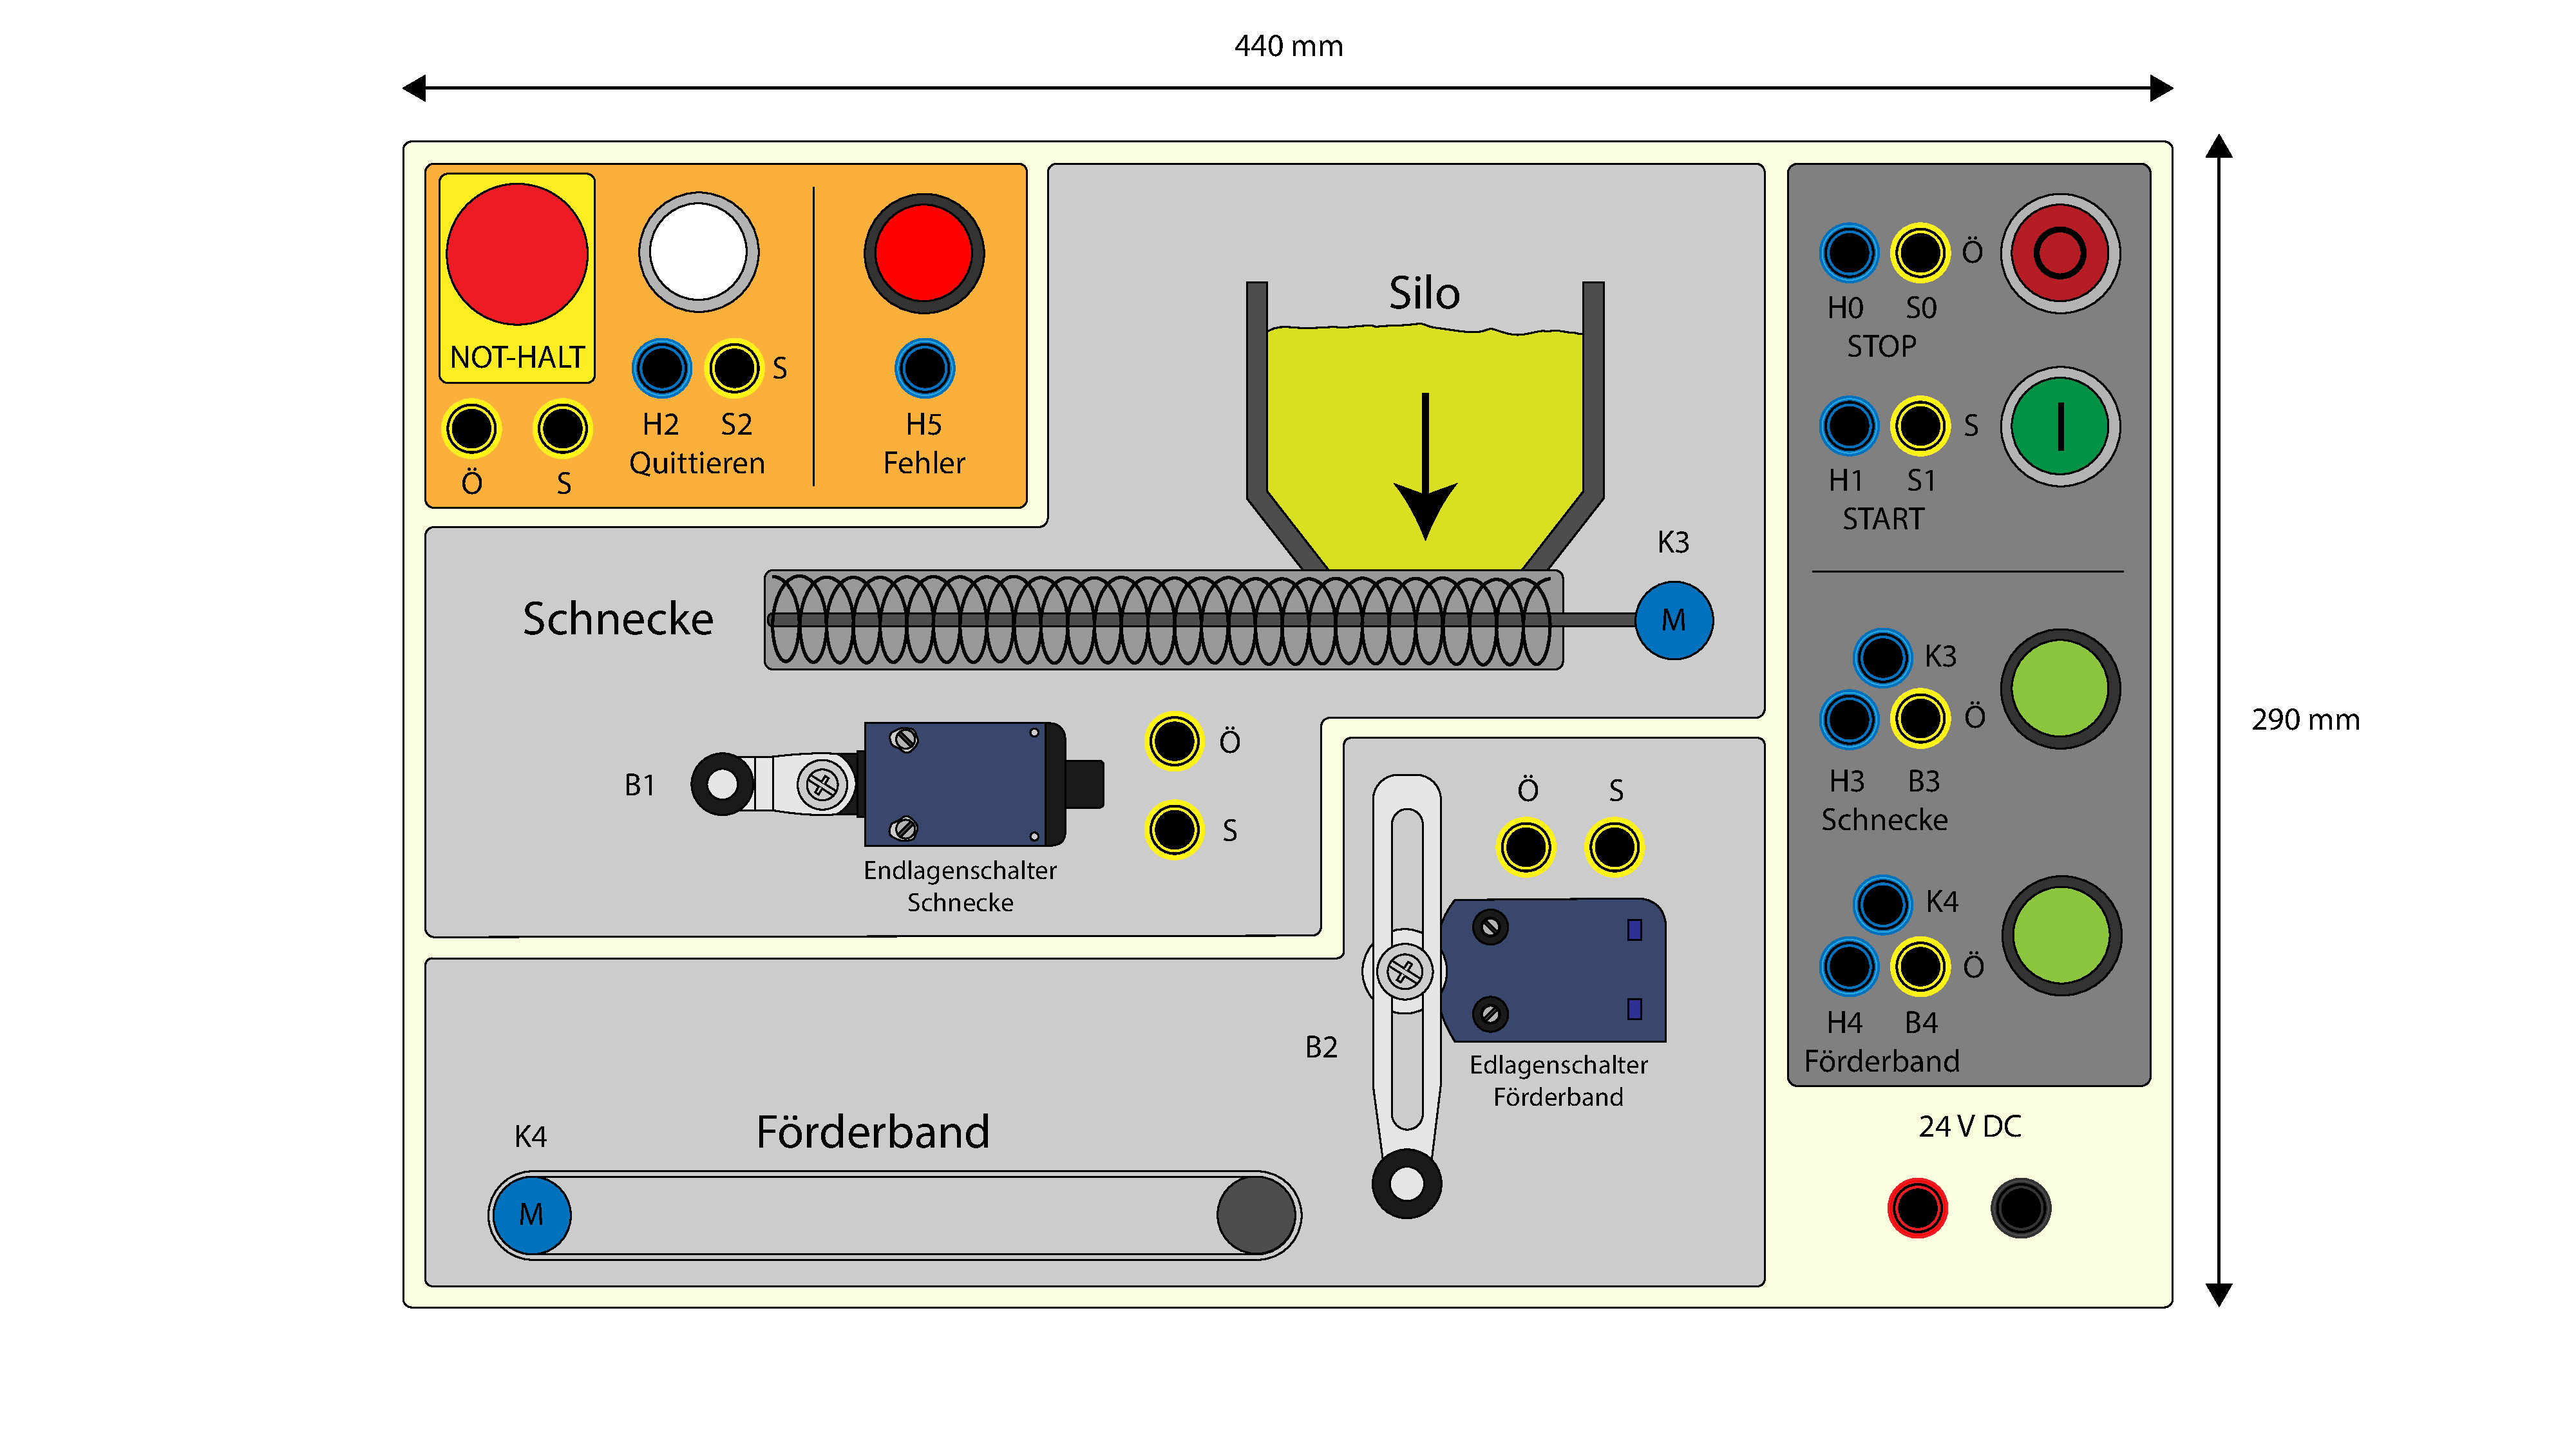
\includegraphics[width=0.95\textwidth]{Bilder/1. Konzept/Aufbauplan_Vorderseite.pdf}}
   \caption[Technologieschema]{Technologisches Schema der Anlage \glqq Silo mit Förderanlage\grqq{}}
   \label{fig:Bild2.1}
\end{figure}

Die Versuchsanlage kann sich grundsätzlich in drei Betriebszustände befinden. Dabei handelt es sich um den \textbf{betriebsbereiten Zustand}, den \textbf{Normalbetrieb} und den \textbf{Fehlerfall}. Diese sind nachfolgend beschrieben.

\subsection{Betriebsbereiter Zustand}

Zunächst muss die Stromversorgung hergestellt werden. Der betriebsbereite Zustand wird erreicht, wenn für die Anlage kein Fehler detektiert wird. Zusätzlich dürfen die Endlagen der Förderschnecke und des Förderbandes (B1, B2) nicht auslösen. Die Motoren müssen ausgeschaltet sein, d.h. die SPS erhält FALSE-Signale der Hilfskontakte (B3, B4) der Schütze (K3, K4).\\
Sind die vorangegangenen Bedingungen erfüllt, blinkt der START-Leuchtdrucktaster (H1) mit einer vorgegeben Frequenz von f = 1 Hz. Der STOP-Leuchtdrucktaster (H0) ist ausgeschaltet.

\subsection{Normalbetrieb}

Die Anlage wird durch das Drücken des START-Leuchtdrucktasters (S1) vom betriebsbereiten Zustand in den Normalbetrieb überführt. Der START-Leuchtdrucktaster (H1) hört zu blinken auf und leuchtet nun dauerhaft. Der STOP-Leuchtdrucktaster (H0) leuchtet ebenfalls dauerhaft. Befindet sich die Anlage im Normalbetrieb, soll der Prozess des Materialtransportes von einer Förderschnecke über ein Förderband simuliert werden. Die Ansteuerung der Förderschnecke und des Förderbandes erfolgt jeweils über eine zugeordnete Motorsteuerung. Die modellhaft dargestellten Motoren werden über Hilfsschütze (K3, K4) angesteuert. Der Schaltzustand der Schütze (B3, B4) wird über Hilfskontakte einerseits zur weiteren Auswertung auf die SPS (S7-1500) rückgeführt, andererseits erfolgt die Signalisierung an den Anwender mittels Leuchtmelder (H3, H4). Damit ein fehlerfreier Transport gewährleistet wird, muss das Förderband vier Sekunden vor der Schnecke anlaufen. Ebenfalls ist ein Nachlauf des Förderbandes von fünf Sekunden nach dem Stoppen der Förderschnecke erforderlich. \\
Die Anlage besitzt sowohl für die Förderschnecke als auch das Förderband einen mechanischen Endlagensensor (B1, B2). Das Erreichen der Endlagen wird der SPS signalisiert. \\
Die Anlage wird durch das Drücken des STOP-Leuchtdrucktasters (S0) angehalten.

\subsection{Fehlerfall}

Tritt ein vom Normalbetrieb abweichender Anlagenzustand auf, wird dieser über die Steuerung bzw. das Steuerungsprogramm erkannt und über das Blinken des FEHLER-Leuchtmelders (H5) signalisiert (Blinktakt 1 Hz). Weiterhin findet ein NOT-Halt statt, so dass keine Gefährdung mehr von der Anlage ausgeht. Ist der Fehler behoben, leuchtet der Fehlerleuchtmelder dauerhaft und der QUITTIER-Leuchtdrucktaster (H2) blinkt mit 1Hz Taktfrequenz. Anschließend muss der Anwender den Fehler mit dem QUITTIER-Taster (S2) quittieren. Aus Sicherheitsgründen sollen sowohl kritische als auch unkritische Fehler quittiert werden. Die Anlage befindet sich nun wieder im betriebsbereiten Zustand. Über das erneute Betätigen des START-Leuchtdrucktasters (S1) nimmt die Anlage ihren Normalbetrieb wieder auf. \\
Es ist möglich verschiedene Fehlersituationen an der Anlage zu simulieren. Diese werden folgendermaßen unterteilt:

\begin{enumerate}
    \item Kritische Fehler
    \begin{itemize}
        \item NOT-Halt Betätigung
        \item Unplausible Sensorsignale
        \item Fehlende Rückmeldung der Motorschütze
        \item Mechanische Blockierung der Endlagensensoren
        \item Abweichung innerhalb eines F-Kanals (Ein-/Ausgänge)
    \end{itemize}
    \item Unkritische Fehler
    \begin{itemize}
        \item Überschreiten der SPS-Zykluszeit (Watchdog-Meldung)
        \item Drahtbruch in der Signalleitung des START- oder STOP-Tasters
        \item Ausfall der SPS (Verlust der Spannungsversorgung)
        \item Förderband läuft nach Schnecke an
        \item Förderband stoppt vor Schnecke
    \end{itemize}
\end{enumerate}

Tritt einer der beschriebenen Fehlerfälle auf, wird die Anlage gestoppt. Es muss erst die Fehlerfreiheit vom Nutzer sichergestellt und quittiert werden, um die Anlage erneut zu starten.

\section{Datenmodell}

Die nachfolgende Datenpunktliste gibt einen Überblick über die zu verwendenden Ein– und Ausgänge:

\begin{table}[H]
    \tiny
    \begin{longtable}{|llllllll|}
        \hline
        \multicolumn{1}{|l|}{\multirow{2}{*}{\textbf{Nr.}}} &
        \multicolumn{1}{l|}{\multirow{2}{*}{\textbf{BMK}}} &
        \multicolumn{1}{l|}{\multirow{2}{*}{\textbf{Text}}} &
        \multicolumn{1}{l|}{\multirow{2}{*}{\textbf{Ort}}} &
        \multicolumn{1}{l|}{\multirow{2}{*}{\textbf{Datentyp}}} &
        \multicolumn{3}{l|}{\textbf{SPS Adr.}} \\ \cline{6-8}
        \multicolumn{1}{|l|}{} & \multicolumn{1}{l|}{} & \multicolumn{1}{l|}{} & \multicolumn{1}{l|}{} &\multicolumn{1}{l|}{} & \multicolumn{1}{l|}{Kanal} & \multicolumn{1}{l|}{Öffner} & Schließer \\ \hline
        \endfirsthead
        %
        \endhead
        %
        \hline
        \endfoot
        %
        \endlastfoot
        %
        %-----------------------------------------------------Normale E/A-----------------------------------------------------------
        \rowcolor{grey}
        \multicolumn{3}{|l}{} & \textbf{Normale E/A} & \multicolumn{4}{l|}{} \\ \hline
        % Eingänge
        \rowcolor{lightGrey}
        & \multicolumn{7}{l|}{\textbf{Eingänge}} \\ \hline
        % S0
        \multicolumn{1}{|l|}{1} & \multicolumn{1}{l|}{S0} & \multicolumn{1}{l|}{STOP-Leuchtdrucktaster} & \multicolumn{1}{l|}{DI 8x24VDC HF} & \multicolumn{1}{l|}{BOOL} & \multicolumn{1}{l|}{} & \multicolumn{1}{l|}{\%I 20.0} & \\
        % S1
        \multicolumn{1}{|l|}{2} & \multicolumn{1}{l|}{S1} & \multicolumn{1}{l|}{START-Leuchtdrucktaster} & \multicolumn{1}{l|}{DI 8x24VDC HF} & \multicolumn{1}{l|}{BOOL} & \multicolumn{1}{l|}{} & \multicolumn{1}{l|}{} & \%I 20.1 \\
        % S2
        \multicolumn{1}{|l|}{3} & \multicolumn{1}{l|}{S2} & \multicolumn{1}{l|}{QUITTIER-Leuchtdrucktaster} & \multicolumn{1}{l|}{DI 8x24VDC HF} & \multicolumn{1}{l|}{BOOL} & \multicolumn{1}{l|}{} & \multicolumn{1}{l|}{} & \%I 20.2 \\
        % B3
        \multicolumn{1}{|l|}{4} & \multicolumn{1}{l|}{B3} & \multicolumn{1}{l|}{Rückmeldung Motorschütz Förderschnecke} & \multicolumn{1}{l|}{DI 8x24VDC HF} & \multicolumn{1}{l|}{BOOL} & \multicolumn{1}{l|}{} & \multicolumn{1}{l|}{} & \%I 20.3 \\
        % B4
        \multicolumn{1}{|l|}{5} & \multicolumn{1}{l|}{B4} & \multicolumn{1}{l|}{Rückmeldung Motorschütz Förderband} & \multicolumn{1}{l|}{DI 8x24VDC HF} & \multicolumn{1}{l|}{BOOL} & \multicolumn{1}{l|}{} & \multicolumn{1}{l|}{} & \%I 20.4 \\ \hline
        % Ausgänge
        \rowcolor{lightGrey}
        & \multicolumn{7}{l|}{\textbf{Ausgänge}} \\ \hline
        % H0
        \multicolumn{1}{|l|}{6} & \multicolumn{1}{l|}{H0} & \multicolumn{1}{l|}{STOP-Leuchtdrucktaster} & \multicolumn{1}{l|}{DQ 8x24VDC/0.5A HF} & \multicolumn{1}{l|}{BOOL} & \multicolumn{1}{l|}{}      & \multicolumn{1}{l|}{} & \%Q 12.0 \\
        % H1
        \multicolumn{1}{|l|}{7} & \multicolumn{1}{l|}{H1} & \multicolumn{1}{l|}{START-Leuchtdrucktaster} & \multicolumn{1}{l|}{DQ 8x24VDC/0.5A HF} & \multicolumn{1}{l|}{BOOL} & \multicolumn{1}{l|}{}      & \multicolumn{1}{l|}{} & \%Q 12.1 \\
        % H2
        \multicolumn{1}{|l|}{8} & \multicolumn{1}{l|}{H2} & \multicolumn{1}{l|}{QUITTIER-Leuchtdrucktaster} & \multicolumn{1}{l|}{DQ 8x24VDC/0.5A HF} & \multicolumn{1}{l|}{BOOL} & \multicolumn{1}{l|}{} & \multicolumn{1}{l|}{} & \%Q 12.2 \\
        % H3
        \multicolumn{1}{|l|}{9} & \multicolumn{1}{l|}{H3} & \multicolumn{1}{l|}{Leuchtmelder Förderschnecke} & \multicolumn{1}{l|}{DQ 8x24VDC/0.5A HF} & \multicolumn{1}{l|}{BOOL} & \multicolumn{1}{l|}{} & \multicolumn{1}{l|}{} & \%Q 12.3 \\
        % H4
        \multicolumn{1}{|l|}{10} & \multicolumn{1}{l|}{H4} & \multicolumn{1}{l|}{Leuchtmelder Förderband} & \multicolumn{1}{l|}{DQ 8x24VDC/0.5A HF} & \multicolumn{1}{l|}{BOOL} & \multicolumn{1}{l|}{}      & \multicolumn{1}{l|}{} & \%Q 12.4 \\ \hline
        %-----------------------------------------------------Fehlersichere E/A-----------------------------------------------------
        \rowcolor{grey}
        \multicolumn{3}{|l}{} & \textbf{Fehlersichere E/A} & \multicolumn{4}{l|}{} \\ \hline
        % Eingänge
        \rowcolor{lightGrey}
        & \multicolumn{7}{l|}{\textbf{Eingänge}} \\ \hline
        % S5
        \multicolumn{1}{|l|}{11} & \multicolumn{1}{l|}{S5} & \multicolumn{1}{l|}{NOT-HALT-Taster} & \multicolumn{1}{l|}{F-DI 8x24VDC HF} & \multicolumn{1}{l|}{BOOL} & \multicolumn{1}{l|}{1}     & \multicolumn{1}{l|}{\%I 22.0} & \%I 23.0 \\
        % B1
        \multicolumn{1}{|l|}{12} & \multicolumn{1}{l|}{B1} & \multicolumn{1}{l|}{Sensor Endlagenschalter Förderschnecke} & \multicolumn{1}{l|}{F-DI 8x24VDC HF} & \multicolumn{1}{l|}{BOOL} & \multicolumn{1}{l|}{2} & \multicolumn{1}{l|}{\%I 22.1} & \%I 23.1 \\
        % B2
        \multicolumn{1}{|l|}{13} & \multicolumn{1}{l|}{B2} & \multicolumn{1}{l|}{Sensor Endlagenschalter Förderband} & \multicolumn{1}{l|}{F-DI 8x24VDC HF} & \multicolumn{1}{l|}{BOOL} & \multicolumn{1}{l|}{3} & \multicolumn{1}{l|}{\%I 22.2} & \%I 23.2 \\ \hline
        % Ausgänge
        \rowcolor{lightGrey}
        & \multicolumn{7}{l|}{\textbf{Ausgänge}} \\ \hline
        % H5
        \multicolumn{1}{|l|}{14} & \multicolumn{1}{l|}{H5} & \multicolumn{1}{l|}{Fehlerleuchtmelder} & \multicolumn{1}{l|}{F-DQ 4x24VDC/2A HF} & \multicolumn{1}{l|}{BOOL} & \multicolumn{1}{l|}{}      & \multicolumn{1}{l|}{} & \%Q 28.0 \\
        % K3
        \multicolumn{1}{|l|}{15} & \multicolumn{1}{l|}{K3} & \multicolumn{1}{l|}{Motorschütz Förderschnecke} & \multicolumn{1}{l|}{F-DQ 4x24VDC/2A HF} & \multicolumn{1}{l|}{BOOL} & \multicolumn{1}{l|}{} & \multicolumn{1}{l|}{} & \%Q 28.1 \\
        % K4
        \multicolumn{1}{|l|}{16} & \multicolumn{1}{l|}{K4} & \multicolumn{1}{l|}{Motorschütz Förderband} & \multicolumn{1}{l|}{F-DQ 4x24VDC/2A HF} & \multicolumn{1}{l|}{BOOL} & \multicolumn{1}{l|}{}      & \multicolumn{1}{l|}{} & \%Q 28.2 \\ \hline
        % Caption
        \caption[Datenmodell des Systems]{Datenmodell des hochverfügbaren und sicheren Systems Silo mit Förderschnecke und Förderband}
        \label{tab:3.1}
    \end{longtable}
\end{table}

Alle Leuchtdrucktaster (S0, S1 und S2) werden an der dezentralen Peripherie ET 200SP sowohl an dem digitalen Eingangsmodul \glqq DI 8x24VDC HF\grqq{} für Schaltbefehle, als auch am digitalen Ausgangsmodul \glqq DQ 8x24VDC/0,5A HF\grqq{} für Leuchtmeldungen (H0, H1, H2) einkanalig angeschlossen. Die Rückmeldungen der Hilfskontakte der Motorschütze (B3 und B4) erfolgen ebenfalls über das Modul \glqq DI 8x24VDC HF\grqq{}. Der Betrieb beider Motoren wird über zugehörige Leuchtmelder (H3 und H4) als Ausgänge des digitalen Ausgangsmodul \glqq DQ 8x24VDC/0,5A HF\grqq{} signalisiert. \\
Die zweikanalig ausgeführten Eingänge (S5, B1, B2) werden an dem fehlersicheren Eingangsmodul \glqq F-DI 8x24VDC HF\grqq{} der dezentralen Peripherie (ET 200SP) betrieben. Der Fehlerleuchtmelder (H5) sowie die Ansteuerung der Motorschütze der Förderschnecke (K3) und des Förderbandes (K4) werden an das fehlersichere Ausgangsmodul \glqq F-DQ 4x24VDC/2.0A HF\grqq{} angeschlossen.

\section{Verhaltensspezifikation}

\begin{figure}[H]
   \centering
   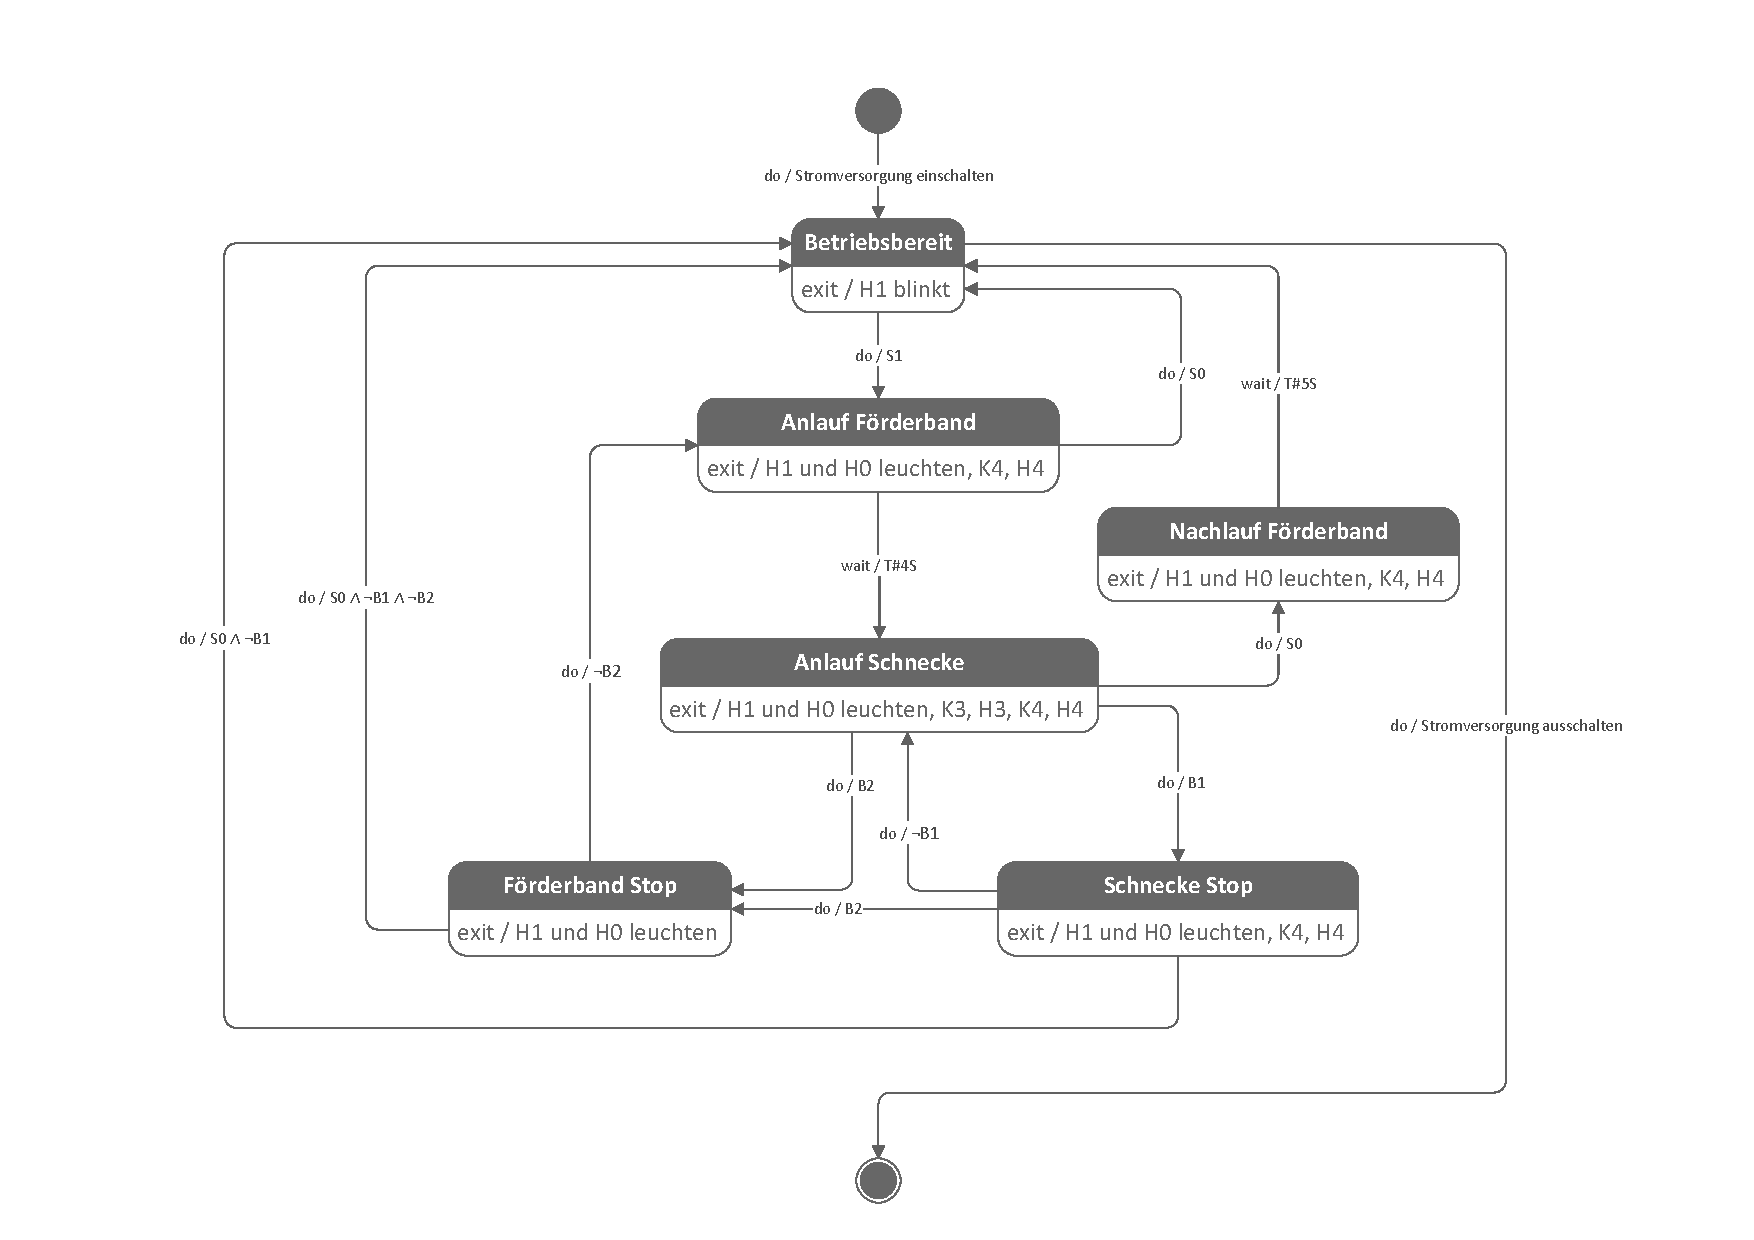
\includegraphics[width=1.0\textwidth]{Bilder/1. Konzept/Normalbetrieb.pdf}
   \caption[Automatengraph Normalbetrieb]{Moore Automatengraph des Normalbetriebs}
   \label{fig:Bild4}
\end{figure}

\begin{figure}[H]
   \centering
   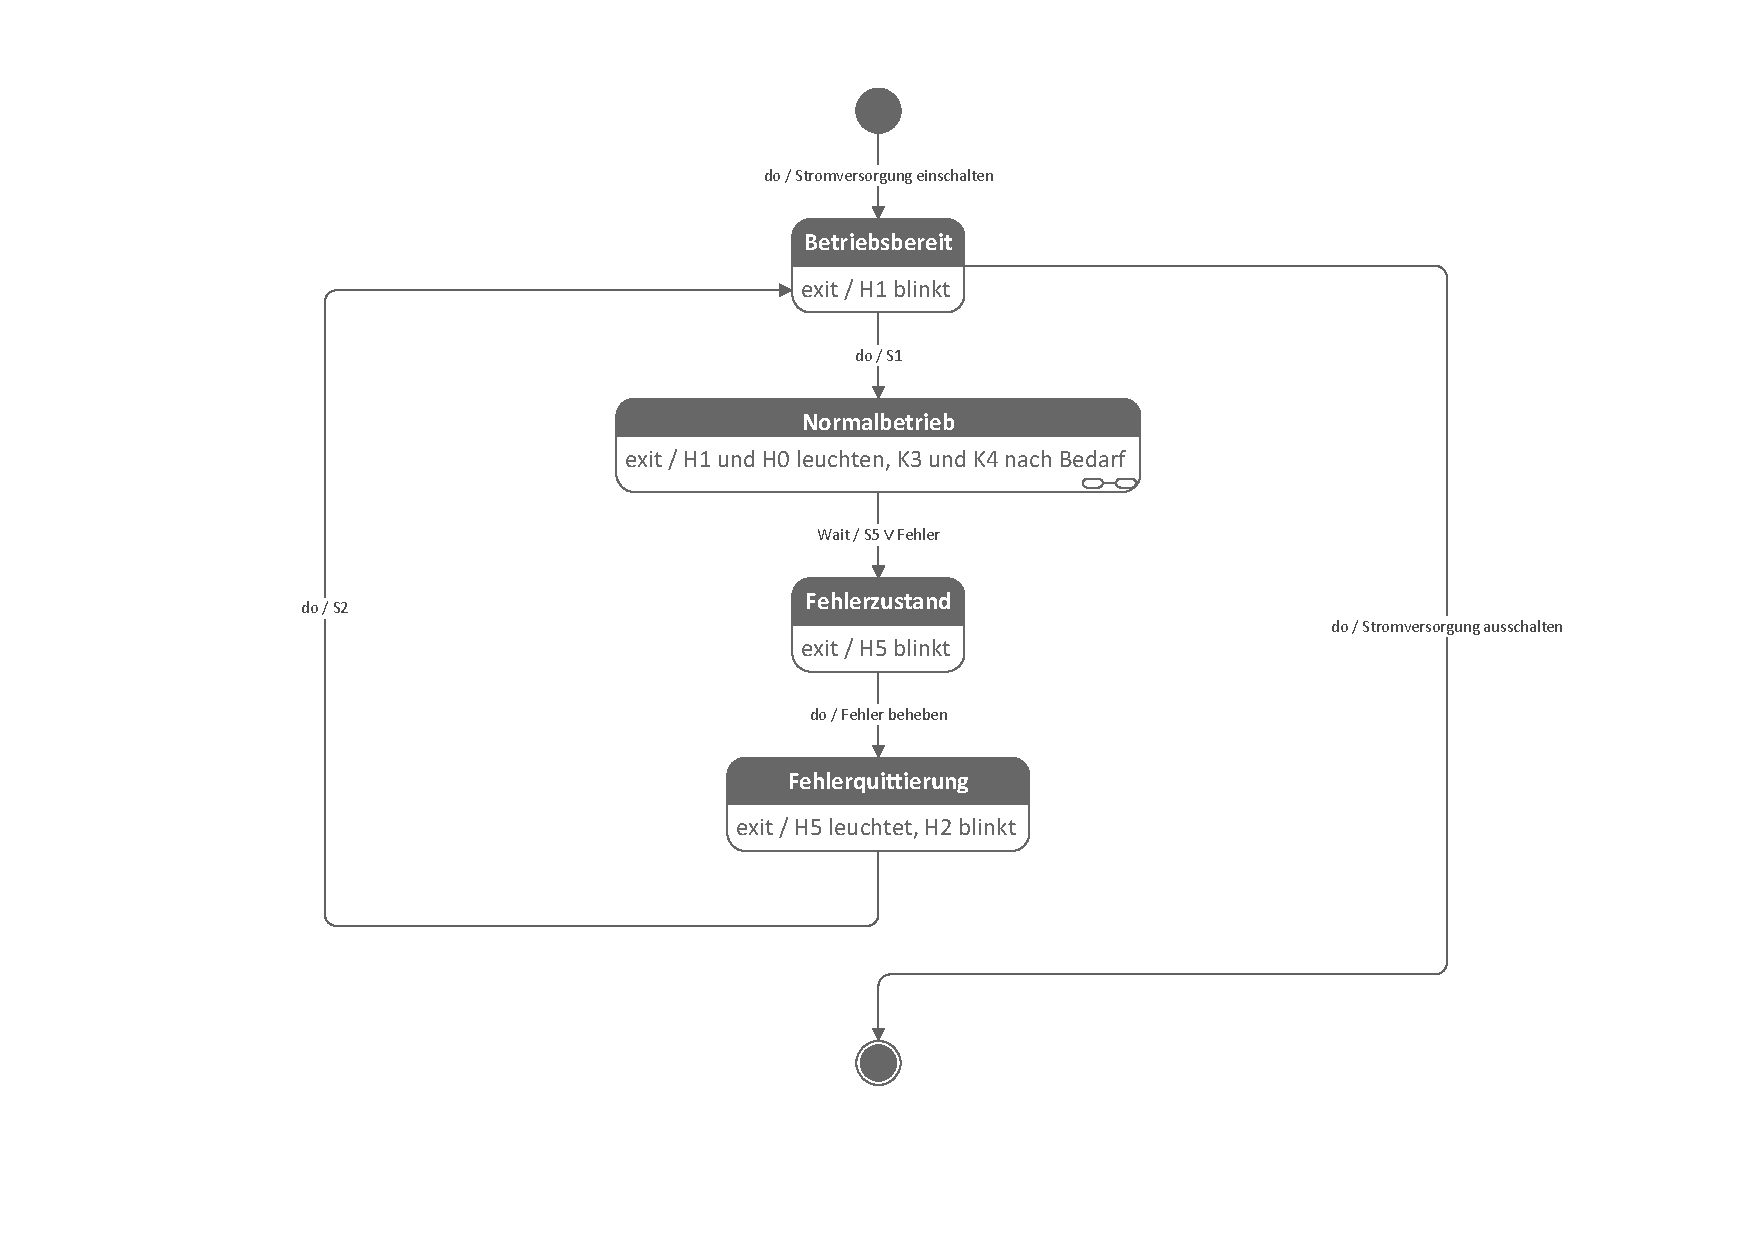
\includegraphics[width=0.8\textwidth]{Bilder/1. Konzept/Fehlerfall.pdf}
   \caption[Automatengraph Fehlerfall]{Moore Automatengraph des Fehlerfalls}
   \label{fig:Bild5}
\end{figure}

\include{5_stromlaufplan.tex}

\section{Inbetriebnahme}

\subsection{Grundlagen}

\subsubsection{Anlagenübersicht}

\begin{figure}[H]
   \centering
   \fbox{\includegraphics[width=0.75\textwidth]{Bilder/2. Inbetriebnahme/1. Grundlagen/(1.1) Anlagenübersicht.png}}
   \caption[Anlagenübersicht]{Anlagenübersicht}
   \label{fig:Bild6.1}
\end{figure}

\begin{figure}[H]
   \centering
   \fbox{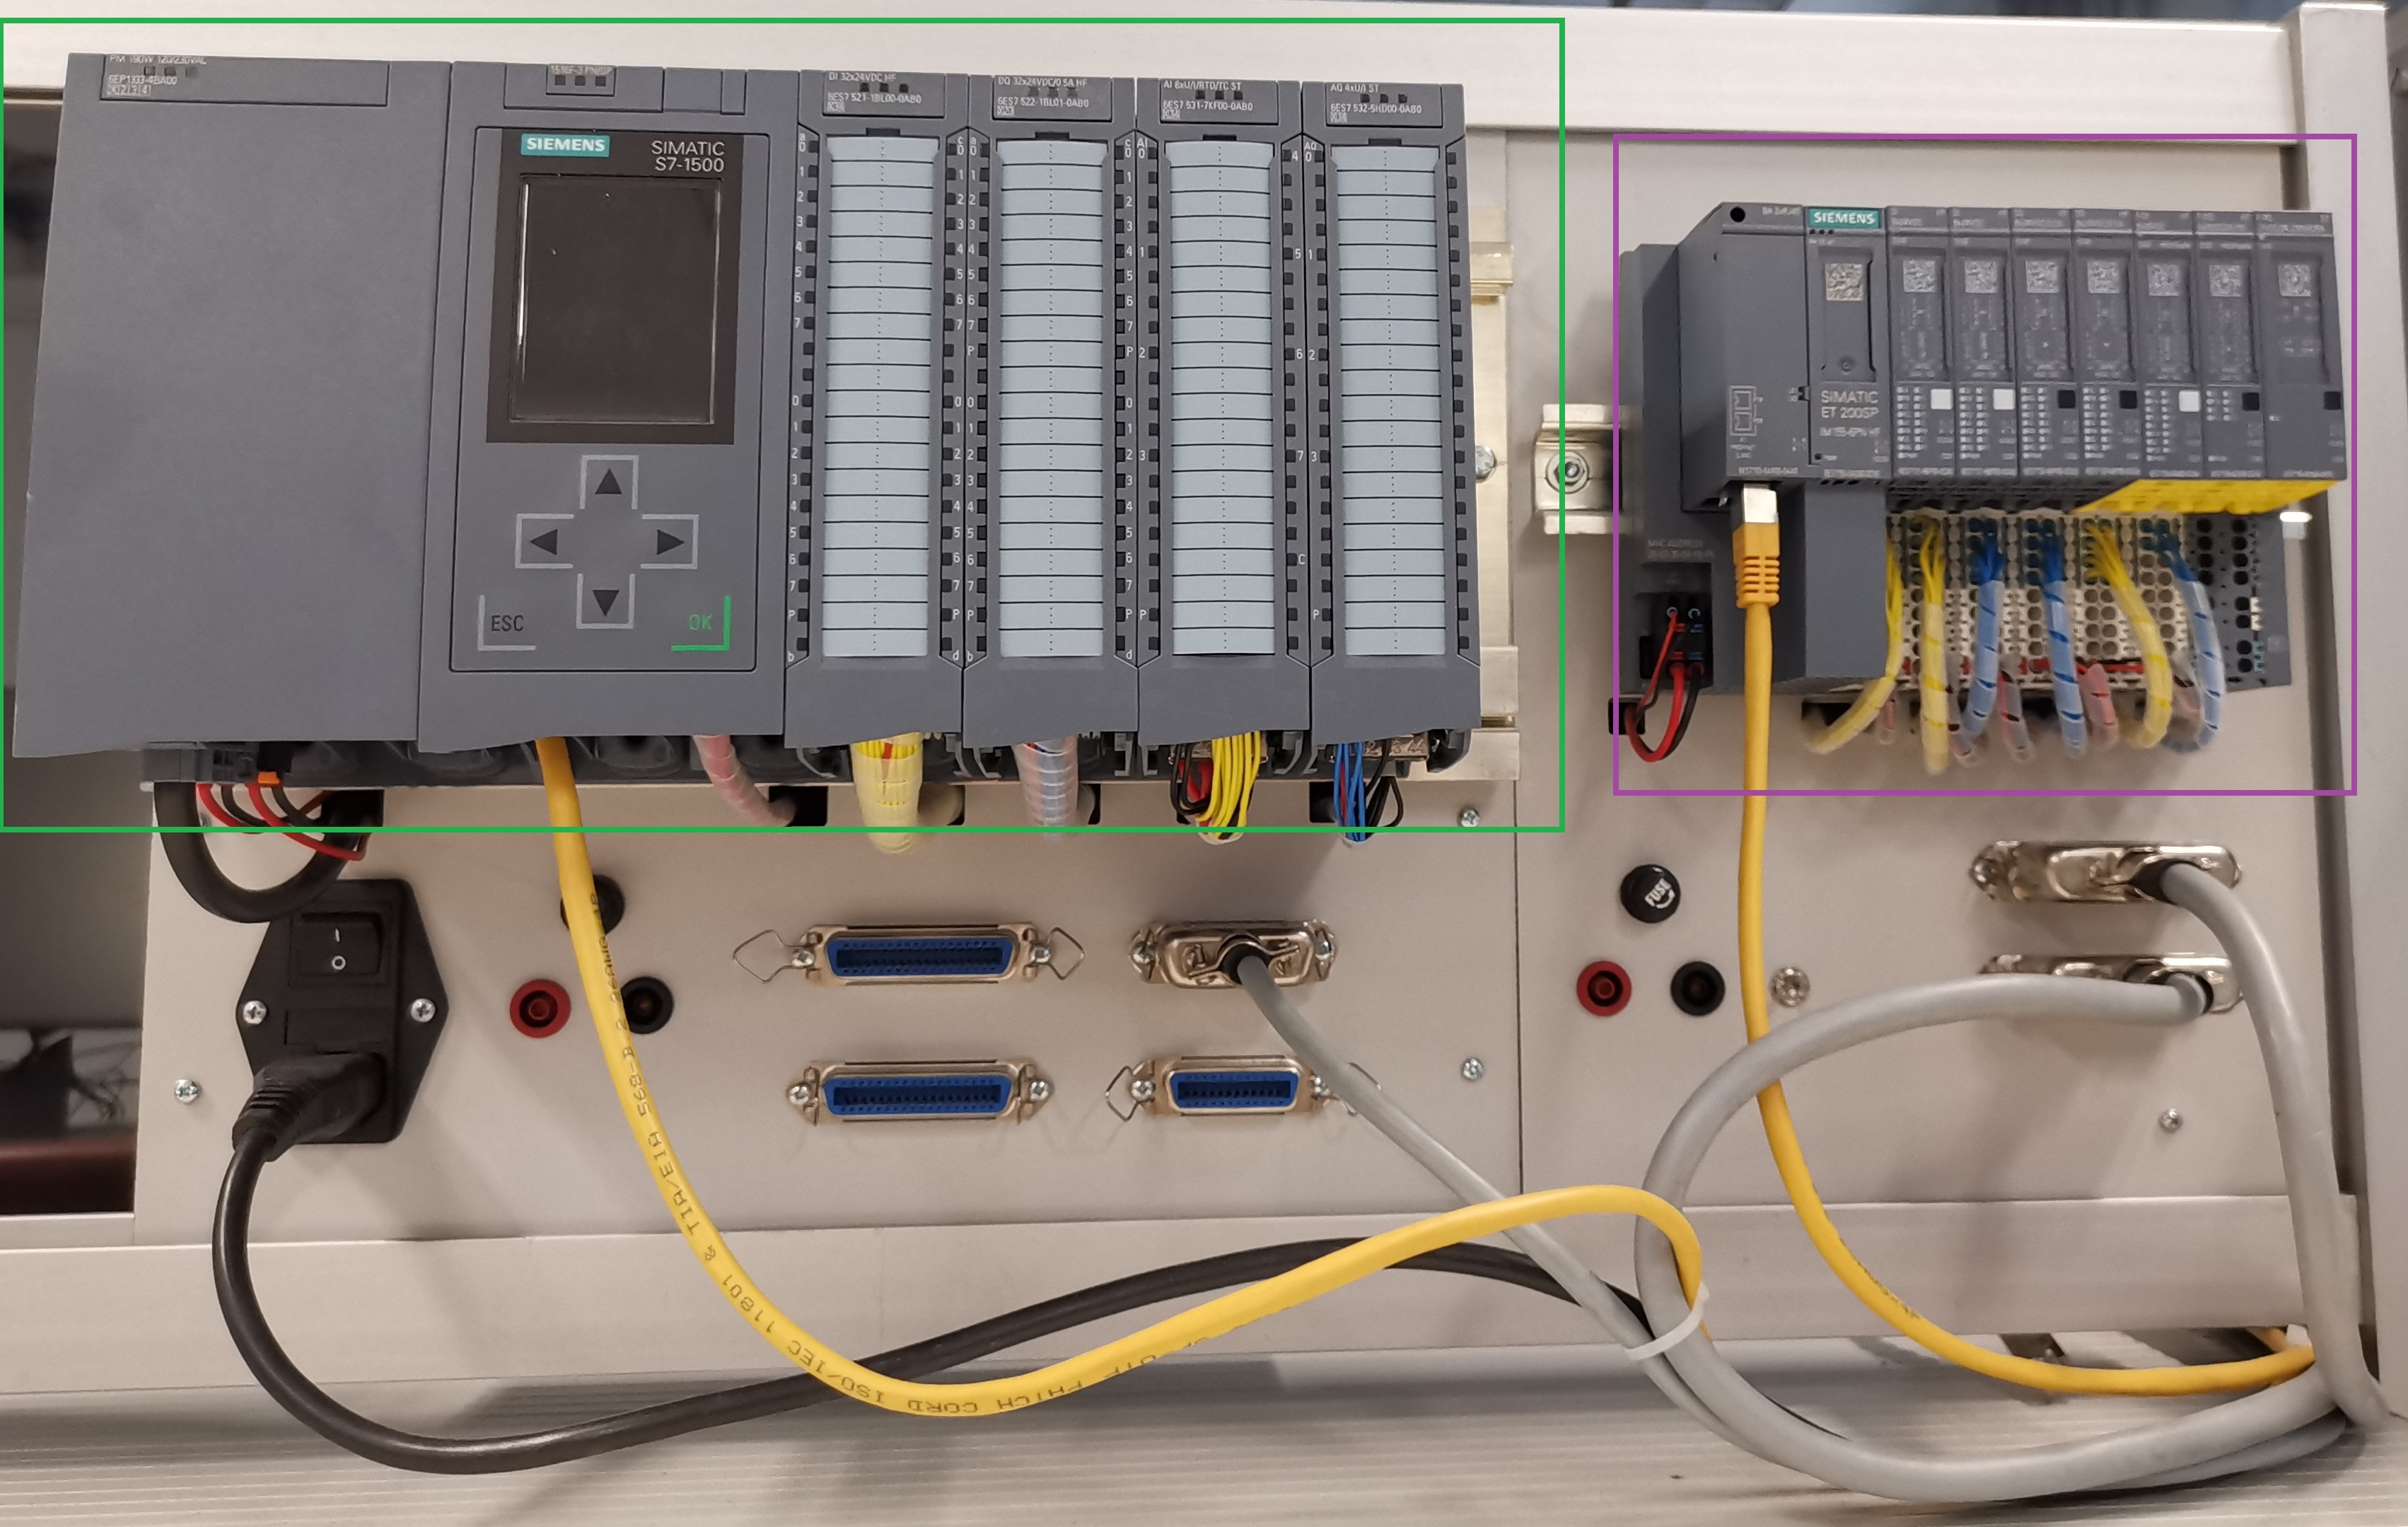
\includegraphics[width=0.75\textwidth]{Bilder/2. Inbetriebnahme/1. Grundlagen/(1.2) Reale Anlage.jpg}}
   \caption[Reale Anlage]{Reale Anlage (links: S7-1500; rechts: ET 200SP)}
   \label{fig:Bild6.2}
\end{figure}

\subsubsection{PROFINET-Gerätenamen und IP-Adressen im Raum WH G-420}
\begin{figure}[H]
    \centering
    \scalebox{0.95}{%
    \begin{tikzpicture}[framed][domain=0:0]
        % Umrandung zeichnen
        \draw[black, very thick] (0,0) rectangle (15,17);
        
        % Eingangstür zeichnen
        \draw[black, very thick](15,0.7) -- (13, 0.7);
        \draw[grey, very thin] (15,2.7) arc (90:180:2);
        
        % Tür zum Büro
        \draw[black, very thick](9, 17) -- (9, 15);
        \draw[grey, very thin] (11, 17) arc (0:-90:2);
        
        % Tafel
        \draw[black, fill = black] (5.5, 0.3) rectangle (9.5, 0.4);
        \draw[black, fill = black] (9.5,0.3) -- (11.5, 1) -- ++(109.29:0.1cm) -- ++(199.29:2.12cm) -- ++(289.29:0.1cm);
        \draw[black, fill = black] (5.5, 0.3) -- (3.5, 1) -- ++(70.71:0.1cm) -- ++(-19.29:2.12cm) -- ++(-109.29:0.1cm);
        
        % Arbeitsplätze Wand
        \draw[black, dashed] (11.3, 2.9) rectangle (14.8, 5.7);
        \draw[black, dashed] (11.3, 5.9) rectangle (14.8, 8.7);
        \draw[black, dashed] (11.3, 8.9) rectangle (14.8, 11.7);
        \draw[black, dashed] (11.3, 11.9) rectangle (14.8, 14.7);
        
        % Arbeitsplätze Fenster
        \draw[black, dashed] (0.2, 2.9) rectangle (3.7, 5.7);
        \draw[black, dashed] (0.2, 5.9) rectangle (3.7, 8.7);
        \draw[black, dashed] (0.2, 8.9) rectangle (3.7, 11.7);
        \draw[black, dashed] (0.2, 11.9) rectangle (3.7, 14.7);
        
        % Arbeitsplätze Gang
        \draw[black, dashed] (3.9, 2.9) rectangle (7.4, 5.7);
        \draw[black, dashed] (3.9, 5.9) rectangle (7.4, 8.7);
        \draw[black, dashed] (3.9, 8.9) rectangle (7.4, 11.7);
        \draw[black, dashed] (3.9, 11.9) rectangle (7.4, 14.7);
        
        % Raum
        \node[font=\bfseries, scale = 1] at (2, 16.5) {Raum WH G-420};
        
        % Subnetz-Text
        \node[scale = 0.8] at (1.9, 16) {Subnetz: 255.255.255.0};
        
        % Gerätenamen PC's & IP-Adressen Fenster
        \node[font=\bfseries, scale = 0.8] at (1.85, 14.4) {FB1-G420-04};
        \node[scale = 0.75] at (1.85, 14) {192.168.1.14};
        \node[font=\bfseries, scale = 0.8] at (1.85, 13.5) {s7-1500-fenster-4};
        \node[scale = 0.75] at (1.85, 13.1) {192.168.1.114};
        \node[font=\bfseries, scale = 0.8] at (1.85, 12.6) {et-200-fenster-4};
        \node[scale = 0.75] at (1.85, 12.2) {192.168.1.134};
        
        \node[font=\bfseries, scale = 0.8] at (1.85, 11.4) {FB1-G420-03};
        \node[scale = 0.75] at (1.85, 11) {192.168.1.13};
        \node[font=\bfseries, scale = 0.8] at (1.85, 10.5) {s7-1500-fenster-3};
        \node[scale = 0.75] at (1.85, 10.1) {192.168.1.113};
        \node[font=\bfseries, scale = 0.8] at (1.85, 9.6) {et-200-fenster-3};
        \node[scale = 0.75] at (1.85, 9.2) {192.168.1.133};
        
        \node[font=\bfseries, scale = 0.8] at (1.85, 8.4) {FB1-G420-02};
        \node[scale = 0.75] at (1.85, 8) {192.168.1.12};
        \node[font=\bfseries, scale = 0.8] at (1.85, 7.5) {s7-1500-fenster-2};
        \node[scale = 0.75] at (1.85, 7.1) {192.168.1.112};
        \node[font=\bfseries, scale = 0.8] at (1.85, 6.6) {et-200-fenster-2};
        \node[scale = 0.75] at (1.85, 6.2) {192.168.1.132};
        
        \node[font=\bfseries, scale = 0.8] at (1.85, 5.4) {FB1-G420-01};
        \node[scale = 0.75] at (1.85, 5) {192.168.1.11};
        \node[font=\bfseries, scale = 0.8] at (1.85, 4.5) {s7-1500-fenster-1};
        \node[scale = 0.75] at (1.85, 4.1) {192.168.1.111};
        \node[font=\bfseries, scale = 0.8] at (1.85, 3.6) {et-200-fenster-1};
        \node[scale = 0.75] at (1.85, 3.2) {192.168.1.131};
        
        % Gerätenamen PC's & IP-Adressen Gang
        \node[font=\bfseries, scale = 0.8] at (5.6, 14.4) {FB1-G420-08};
        \node[scale = 0.75] at (5.6, 14) {192.168.1.18};
        \node[font=\bfseries, scale = 0.8] at (5.6, 13.5) {s7-1500-gang-4};
        \node[scale = 0.75] at (5.6, 13.1) {192.168.1.118};
        \node[font=\bfseries, scale = 0.8] at (5.6, 12.6) {et-200-gang-4};
        \node[scale = 0.75] at (5.6, 12.2) {192.168.1.138};
        
        \node[font=\bfseries, scale = 0.8] at (5.6, 11.4) {FB1-G420-07};
        \node[scale = 0.75] at (5.6, 11) {192.168.1.17};
        \node[font=\bfseries, scale = 0.8] at (5.6, 10.5) {s7-1500-gang-3};
        \node[scale = 0.75] at (5.6, 10.1) {192.168.1.117};
        \node[font=\bfseries, scale = 0.8] at (5.6, 9.6) {et-200-gang-3};
        \node[scale = 0.75] at (5.6, 9.2) {192.168.1.137};
        
        \node[font=\bfseries, scale = 0.8] at (5.6, 8.4) {FB1-G420-06};
        \node[scale = 0.75] at (5.6, 8) {192.168.1.16};
        \node[font=\bfseries, scale = 0.8] at (5.6, 7.5) {s7-1500-gang-2};
        \node[scale = 0.75] at (5.6, 7.1) {192.168.1.116};
        \node[font=\bfseries, scale = 0.8] at (5.6, 6.6) {et-200-gang-2};
        \node[scale = 0.75] at (5.6, 6.2) {192.168.1.136};
        
        \node[font=\bfseries, scale = 0.8] at (5.6, 5.4) {FB1-G420-05};
        \node[scale = 0.75] at (5.6, 5) {192.168.1.15};
        \node[font=\bfseries, scale = 0.8] at (5.6, 4.5) {s7-1500-gang-1};
        \node[scale = 0.75] at (5.6, 4.1) {192.168.1.115};
        \node[font=\bfseries, scale = 0.8] at (5.6, 3.6) {et-200-gang-1};
        \node[scale = 0.75] at (5.6, 3.2) {192.168.1.135};
        
        % Gerätenamen PC's & IP-Adressen Wand
        \node[font=\bfseries, scale = 0.8] at (13, 14.4) {FB1-G420-12};
        \node[scale = 0.75] at (13, 14) {192.168.1.22};
        \node[font=\bfseries, scale = 0.8] at (13, 13.5) {s7-1500-wand-4};
        \node[scale = 0.75] at (13, 13.1) {192.168.1.122};
        \node[font=\bfseries, scale = 0.8] at (13, 12.6) {et-200-wand-4};
        \node[scale = 0.75] at (13, 12.2) {192.168.1.142};
        
        \node[font=\bfseries, scale = 0.8] at (13, 11.4) {FB1-G420-11};
        \node[scale = 0.75] at (13, 11) {192.168.1.21};
        \node[font=\bfseries, scale = 0.8] at (13, 10.5) {s7-1500-wand-3};
        \node[scale = 0.75] at (13, 10.1) {192.168.1.121};
        \node[font=\bfseries, scale = 0.8] at (13, 9.6) {et-200-wand-3};
        \node[scale = 0.75] at (13, 9.2) {192.168.1.141};
        
        \node[font=\bfseries, scale = 0.8] at (13, 8.4) {FB1-G420-10};
        \node[scale = 0.75] at (13, 8) {192.168.1.20};
        \node[font=\bfseries, scale = 0.8] at (13, 7.5) {s7-1500-wand-2};
        \node[scale = 0.75] at (13, 7.1) {192.168.1.120};
        \node[font=\bfseries, scale = 0.8] at (13, 6.6) {et-200-wand-2};
        \node[scale = 0.75] at (13, 6.2) {192.168.1.140};
        
        \node[font=\bfseries, scale = 0.8] at (13, 5.4) {FB1-G420-09};
        \node[scale = 0.75] at (13, 5) {192.168.1.19};
        \node[font=\bfseries, scale = 0.8] at (13, 4.5) {s7-1500-wand-1};
        \node[scale = 0.75] at (13, 4.1) {192.168.1.119};
        \node[font=\bfseries, scale = 0.8] at (13, 3.6) {et-200-wand-1};
        \node[scale = 0.75] at (13, 3.2) {192.168.1.139};
    \end{tikzpicture}%
    }
    \caption[IP-Adressen und PROFINET-Gerätenamen im Raum WH G-420]{IP-Adressen und PROFINET-Gerätenamen im Raum WH G-420}
    \label{fig:Bild6.3}
\end{figure}

\subsection{Neues Projekt anlegen} \label{sec: Neues_Projekt_anlegen}

\subsubsection{TIA Portal öffnen}

Im PC-Menü \glqq\textbf{Start}\grqq\:nach dem \textbf{TIA Portal} suchen (hier Version: V17) und Software starten.
\begin{figure}[H]
   \centering
   \fbox{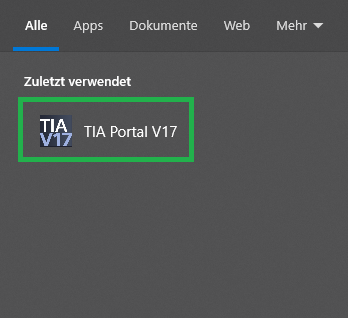
\includegraphics[width=0.4\textwidth]{Bilder/2. Inbetriebnahme/2. Neues Projekt anlegen/(2.1) TIA Portal V17 oeffnen.png}}
   \caption[TIA Portal öffnen]{TIA Portal öffnen}
   \label{fig:Bild6.4}
\end{figure}

\subsubsection{Projekt erstellen}

\textbf{Projektname, Pfad} und \textbf{Autor} des neuen Projektes vergeben und mit \glqq\textbf{Erstellen}\grqq\:bestätigen.
\begin{figure}[H]
   \centering
   \fbox{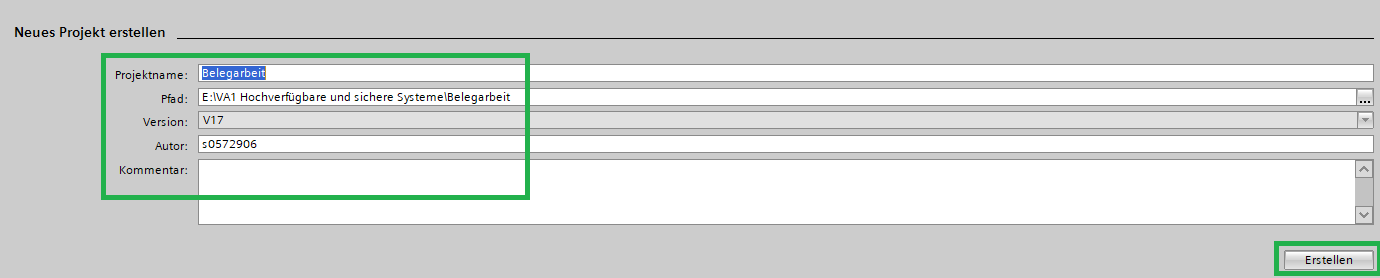
\includegraphics[width=0.95\textwidth]{Bilder/2. Inbetriebnahme/2. Neues Projekt anlegen/(2.2) Neues Projekt erstellen.png}}
   \caption[Neues Projekt erstellen]{Neues Projekt erstellen}
   \label{fig:Bild6.5}
\end{figure}

\clearpage

\subsubsection{Projektansicht öffnen}

Die Projektansicht über \glqq\textbf{Projektansicht öffnen}\grqq\:aufrufen und weitere Einstellungen vornehmen.
\begin{figure}[H]
   \centering
   \fbox{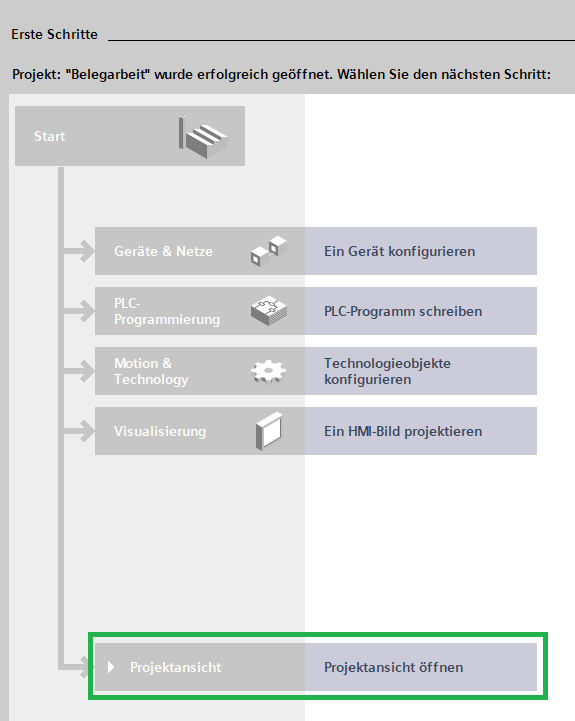
\includegraphics[width=0.6\textwidth]{Bilder/2. Inbetriebnahme/2. Neues Projekt anlegen/(2.3) Projektansicht oeffnen.png}}
   \caption[Projektansicht öffnen]{Projektansicht öffnen}
   \label{fig:Bild6.6}
\end{figure}

\clearpage

\subsection{Konfiguration der S7-1500} \label{sec: Konfiguration_der_S7_1500}

\subsubsection{S7-1500 hinzufügen}
Über \glqq\textbf{Neues Gerät hinzufügen}\grqq\:nach \textbf{6ES7 5XX-XXXXX-XXXX} suchen und mit \glqq\textbf{OK}\grqq\:bestätigen.\\
Pfad: Controller > SIMATIC S7-1500 > CPU > Nicht spezifizierte CPU 1500
\begin{figure}[H]
    \centering
   \begin{minipage}[b]{.4\linewidth}
        \centering
        \fbox{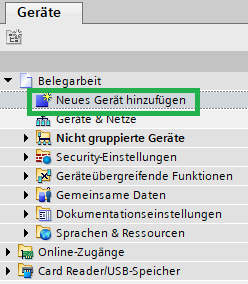
\includegraphics[width=1\linewidth]{Bilder/2. Inbetriebnahme/3. Konfiguration der S7-1500/3.1 S7-1500 hinzufügen/(3.1.1) Neues Geraet hinzufuegen.png}}
        \caption[Neues Gerät hinzufügen]{Neues Gerät hinzufügen}
        \label{fig:Bild6.7}
   \end{minipage}
   \hspace{.1\linewidth}% Abstand zwischen Bilder
   \begin{minipage}[b]{.4\linewidth}
        \centering
        \fbox{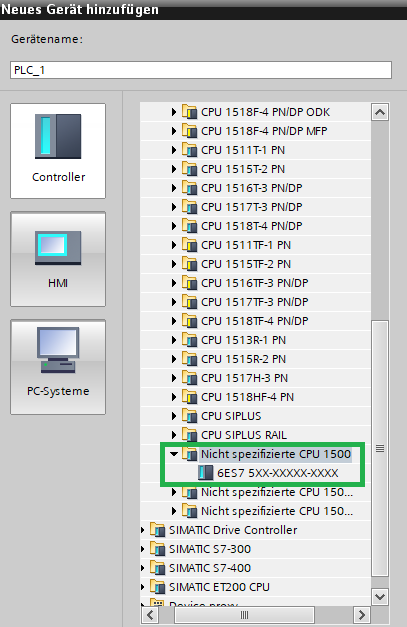
\includegraphics[width=1\linewidth]{Bilder/2. Inbetriebnahme/3. Konfiguration der S7-1500/3.1 S7-1500 hinzufügen/(3.1.2) SPS auswaehlen.png}}
        \caption[S7-1500 auswählen]{S7-1500 auswählen}
        \label{fig:Bild6.8}
   \end{minipage}
\end{figure}

\clearpage

\subsubsection{Kommunikation herstellen}
In der \textbf{Gerätesicht} der S7-1500 über \glqq\textbf{ermitteln}\grqq\:die entsprechende Hardware suchen.
\begin{figure}[H]
   \centering
   \fbox{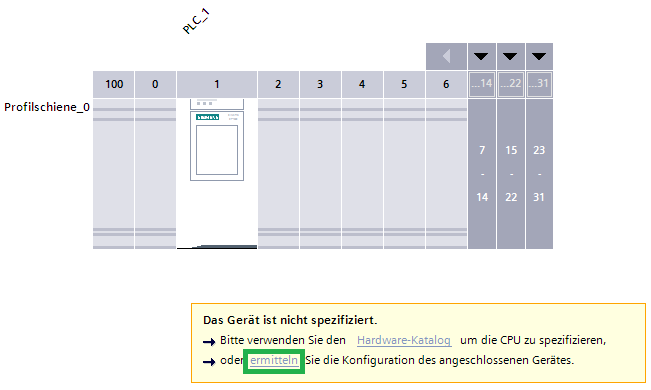
\includegraphics[width=0.7\textwidth]{Bilder/2. Inbetriebnahme/3. Konfiguration der S7-1500/3.2 Kommunikation herstellen/(3.2.1) Hardware ermitteln.png}}
   \caption[Hardware ermitteln]{Hardware ermitteln}
   \label{fig:Bild6.9}
\end{figure}

Einstellungen der Schnittstelle vornehmen und mit \glqq\textbf{Suche starten}\grqq\:nach Geräten suchen. Anschließend das richtige Gerät anhand der IP-Adresse (hier: 192.168.1.116) auswählen und mit \glqq\textbf{Erkennen}\grqq\:bestätigen.
\begin{figure}[H]
   \centering
   \fbox{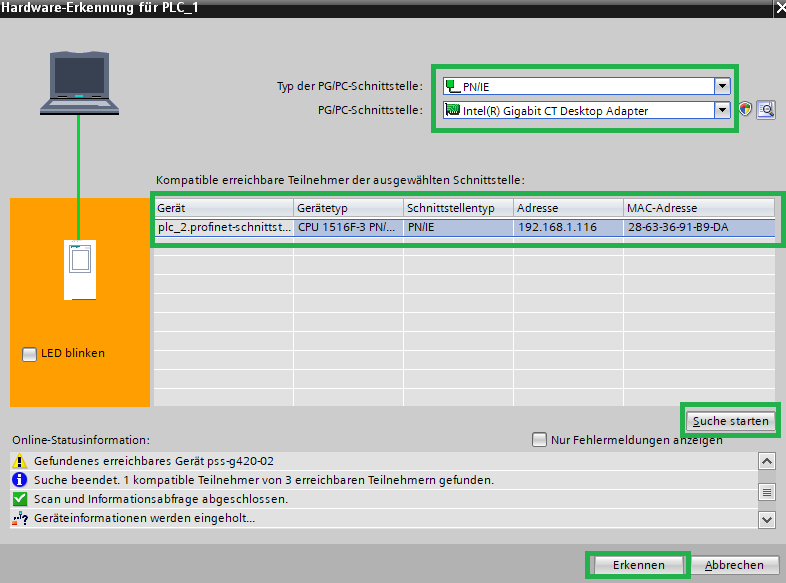
\includegraphics[width=0.6\textwidth]{Bilder/2. Inbetriebnahme/3. Konfiguration der S7-1500/3.2 Kommunikation herstellen/(3.2.2) Kommunikation aufnehmen.png}}
   \caption[Kommunikation herstellen]{Kommunikation herstellen}
   \label{fig:Bild6.10}
\end{figure}

Da das Gerät erstmalig hinzugefügt wurde, ist es sinnvoll, dies als vertrauenswürdig einzustufen (\autoref{fig:Bild6.11}). Die gemachten Einstellungen sollen nicht als Voreinstellungen übernommen werden (\autoref{fig:Bild6.12}).  
\begin{figure}[H]
   \centering
   \fbox{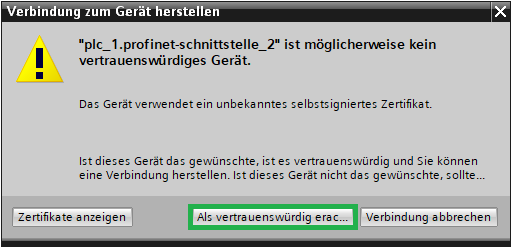
\includegraphics[width=0.75\textwidth]{Bilder/2. Inbetriebnahme/3. Konfiguration der S7-1500/3.2 Kommunikation herstellen/(3.2.3) Vertrauenswuerdigkeit zulassen.PNG}}
   \caption[Gerät als vertrauenswürdig einstufen]{Gerät als vertrauenswürdig einstufen}
   \label{fig:Bild6.11}
\end{figure}

\begin{figure}[H]
   \centering
   \fbox{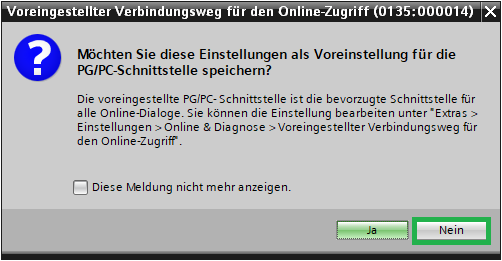
\includegraphics[width=0.75\textwidth]{Bilder/2. Inbetriebnahme/3. Konfiguration der S7-1500/3.2 Kommunikation herstellen/(3.2.4) Voreinstellungen nicht zulassen.PNG}}
   \caption[Nicht als Voreinstellung übernehmen]{Nicht als Voreinstellung übernehmen}
   \label{fig:Bild6.12}
\end{figure}

\clearpage

\subsubsection{Security-Einstellungen der S7-1500}
Nachdem das Gerät erkannt wurde, öffnet sich das Fenster \textbf{PLC Security-Einstellungen}.\\
\textbf{ACHTUNG}: Dies hängt von der Version der S7-1500 ab.\\
\newline
1. Schutz vertraulicher PLC-Konfigurationsdaten \textbf{deaktivieren}:
\begin{figure}[H]
   \centering
   \fbox{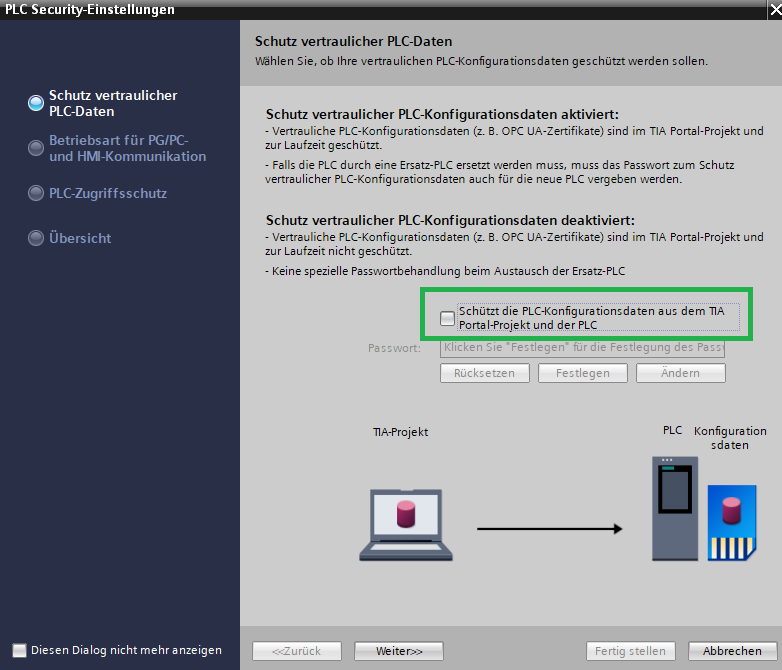
\includegraphics[width=0.8\textwidth]{Bilder/2. Inbetriebnahme/3. Konfiguration der S7-1500/3.3 Security-Einstellungen der S7-1500/(3.3.1) Security Einstellungen (1).png}}
   \caption[Security Einstellungen Teil 1]{Security Einstellungen Teil 1}
   \label{fig:Bild6.13}
\end{figure}

\clearpage

2. Legacy- und Secure PG/PC-Kommunikation \textbf{nicht zulassen}:
\begin{figure}[H]
   \centering
   \fbox{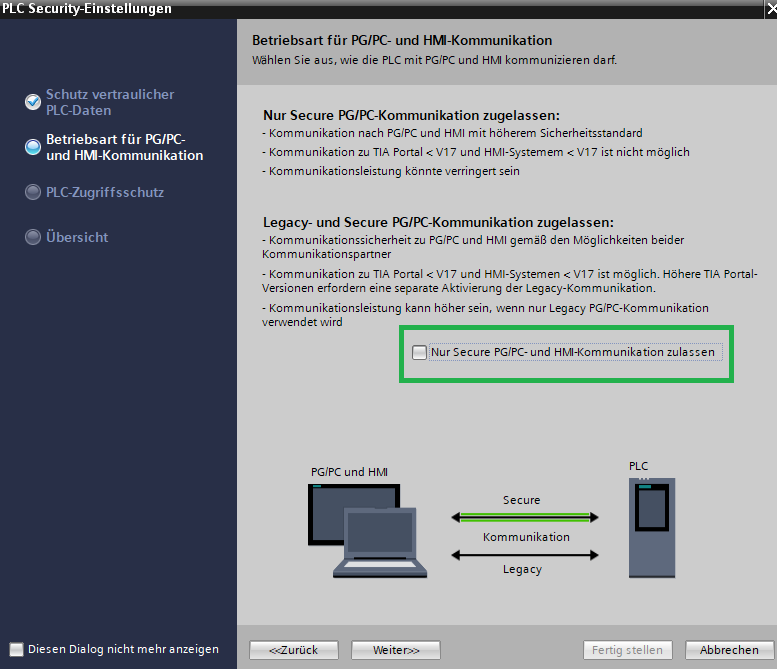
\includegraphics[width=0.8\textwidth]{Bilder/2. Inbetriebnahme/3. Konfiguration der S7-1500/3.3 Security-Einstellungen der S7-1500/(3.3.2) Security Einstellungen (2).png}}
   \caption[Security Einstellungen Teil 2]{Security Einstellungen Teil 2}
   \label{fig:Bild6.14}
\end{figure}

\clearpage

3. Zugriffstufe ohne Passwort auf \textbf{Vollzugriff inkl. fehlersicher (kein Schutz)} stellen:
\begin{figure}[H]
   \centering
   \fbox{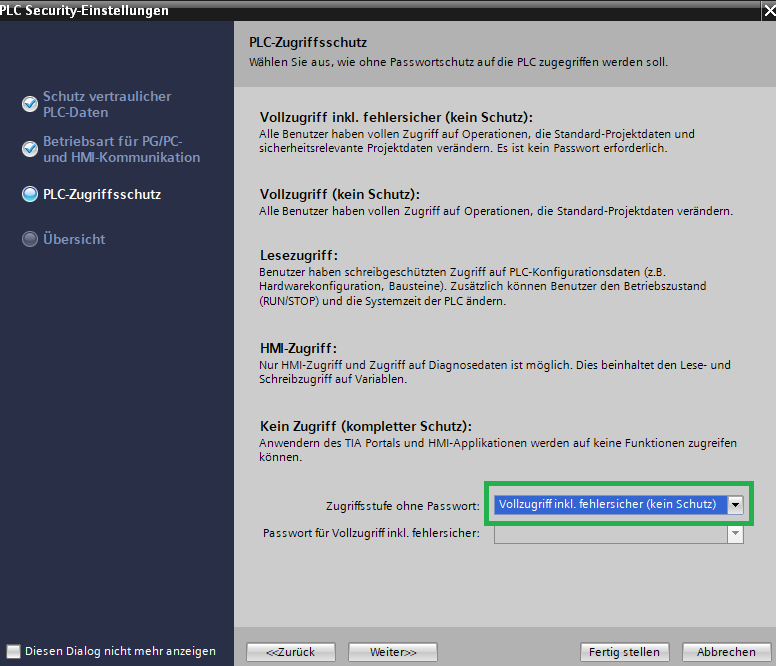
\includegraphics[width=0.8\textwidth]{Bilder/2. Inbetriebnahme/3. Konfiguration der S7-1500/3.3 Security-Einstellungen der S7-1500/(3.3.3) Security Einstellungen (3).png}}
   \caption[Security Einstellungen Teil 3]{Security Einstellungen Teil 3}
   \label{fig:Bild6.15}
\end{figure}

Die Einstellungen mit \glqq\textbf{Fertig stellen}\grqq\:übernehmen. Zuletzt über die \textbf{Gerätesicht} der S7-1500 den \textbf{Schreibzugriff deaktivieren}.\\
Pfad: Allgemein > Display > Passwort 
\begin{figure}[H]
   \centering
   \fbox{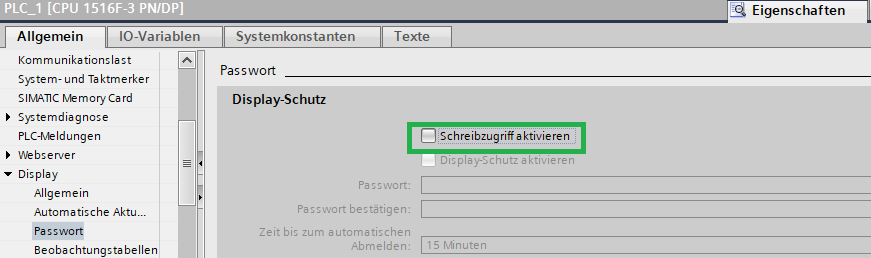
\includegraphics[width=0.8\textwidth]{Bilder/2. Inbetriebnahme/3. Konfiguration der S7-1500/3.3 Security-Einstellungen der S7-1500/(3.3.4) Passwortschutz entfernen.png}}
   \caption[Passwortschutz entfernen]{Passwortschutz entfernen}
   \label{fig:Bild6.16}
\end{figure}

\clearpage

\subsubsection{IP-Adresse und Vergabe des PROFINET-Gerätenamen der S7-1500} \label{sec: IP-Adresse_PROFINET-Gerätename_S7-1500}
Die jeweiligen IP-Adressen und PROFINET-Gerätenamen können der \autoref{fig:Bild6.3} entnommen werden. Die Bezeichnung des PROFINET-Anschlusses ist \textbf{X2}.

\begin{figure}[H]
   \centering
   \fbox{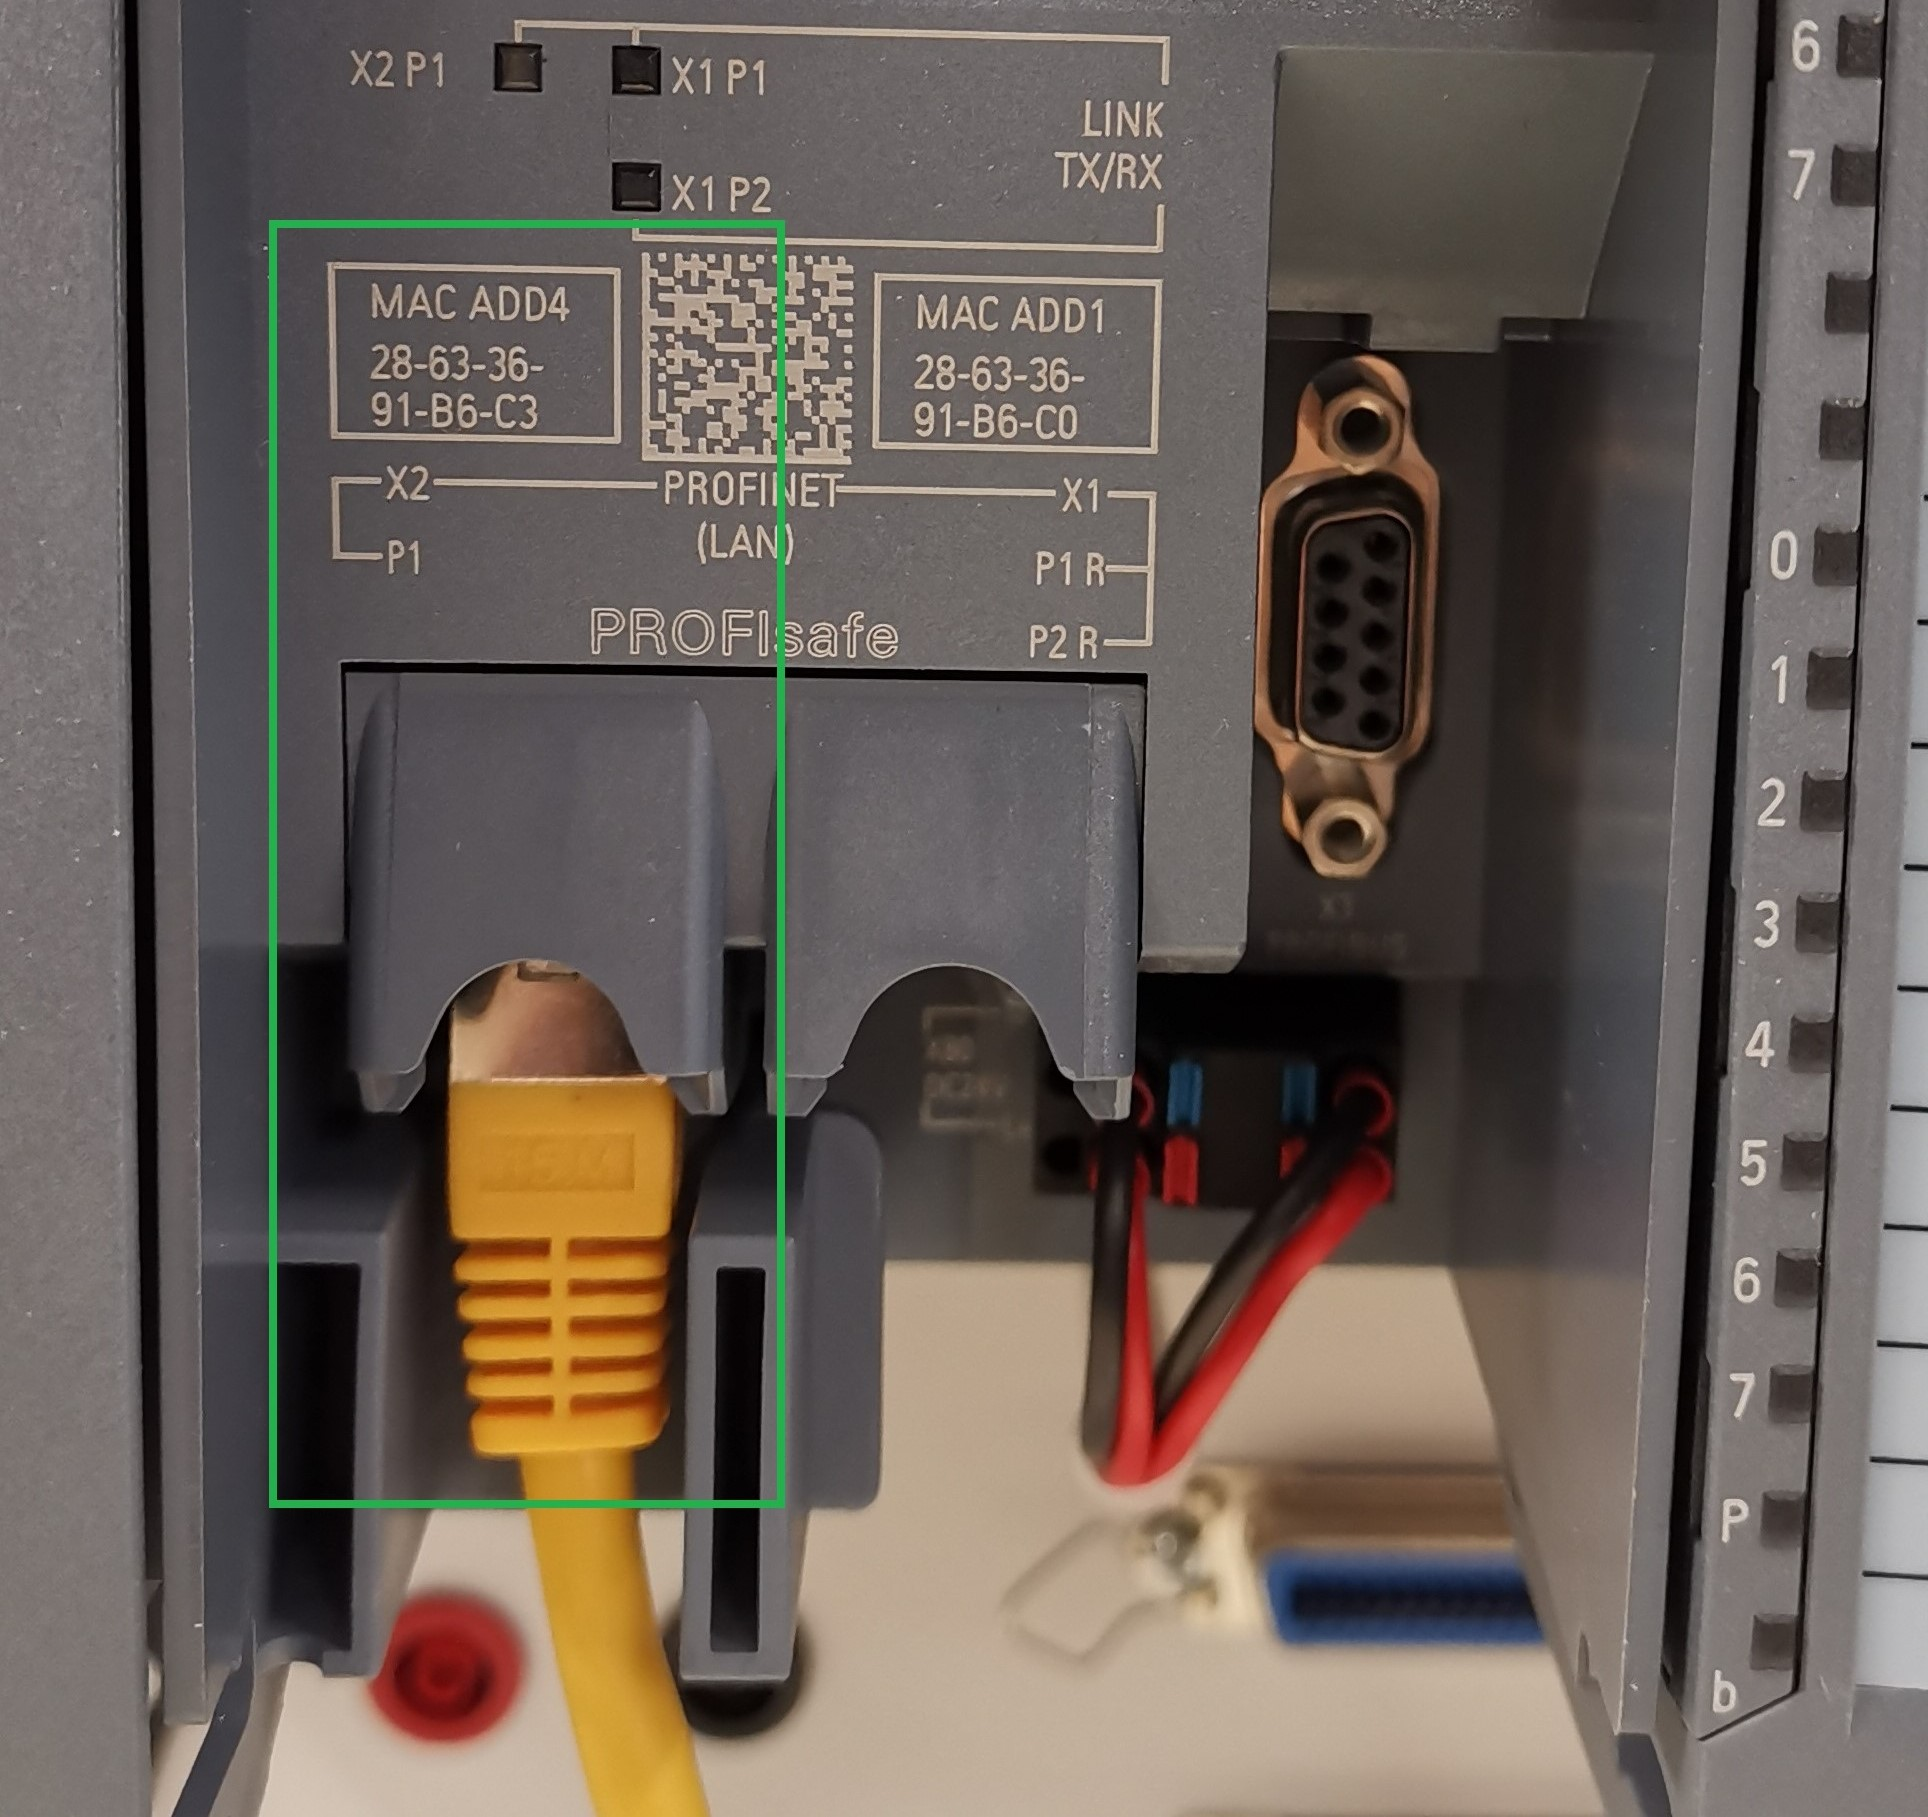
\includegraphics[width=0.45\textwidth]{Bilder/2. Inbetriebnahme/3. Konfiguration der S7-1500/3.4 IP-Adresse und Vergabe des PROFINET-Gerätenamen der S7-1500/(3.4.1) PROFINET-Schnittstelle.jpg}}
   \caption[Anschluss an PROFINET-Schnittstelle]{Anschluss an PROFINET-Schnittstelle}
   \label{fig:Bild6.17}
\end{figure}

1. IP-Adresse vergeben:\\
Pfad über \textbf{Gerätesicht}: Allgemein > PROFINET-Schnittstelle [X2] > Ethernet-Adressen
\begin{figure}[H]
   \centering
   \fbox{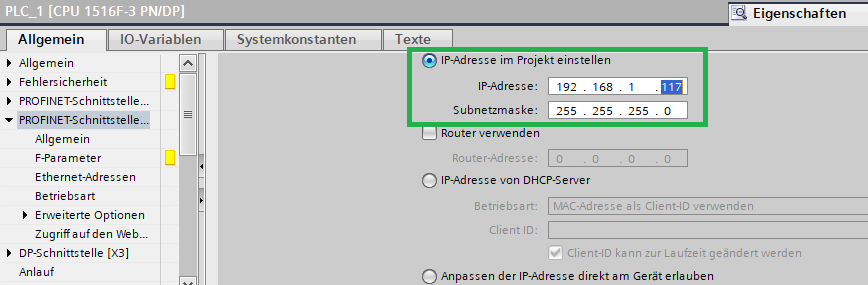
\includegraphics[width=0.9\textwidth]{Bilder/2. Inbetriebnahme/3. Konfiguration der S7-1500/3.4 IP-Adresse und Vergabe des PROFINET-Gerätenamen der S7-1500/(3.4.2) IP-Adresse der S7 einstellen.png}}
   \caption[IP-Adresse der S7-1500 eingeben]{IP-Adresse der S7-1500 eingeben}
   \label{fig:Bild6.18}
\end{figure}

\clearpage

2. PROFINET-Gerätename vergeben:\\
Pfad über \textbf{Gerätesicht}: Allgemein > PROFINET-Schnittstelle [X2] > Ethernet-Adressen\\
\newline
Zur Eingabe des PROFINET-Gerätenamen das Häkchen bei \glqq\textbf{PROFINET-Gerätename automatisch generieren}\grqq\:entfernen.

\begin{figure}[H]
   \centering
   \fbox{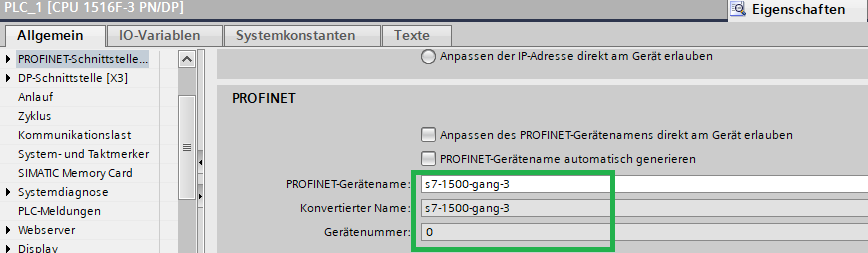
\includegraphics[width=0.9\textwidth]{Bilder/2. Inbetriebnahme/3. Konfiguration der S7-1500/3.4 IP-Adresse und Vergabe des PROFINET-Gerätenamen der S7-1500/(3.4.3) PROFINET-Geraetename S7 einstellen.png}}
   \caption[PROFINET-Gerätename der S7-1500 eingeben]{PROFINET-Gerätename der S7-1500 eingeben}
   \label{fig:Bild6.19}
\end{figure}

\clearpage

\subsection{Konfiguration der ET 200SP} \label{sec:Konfiguration_der_ET_200_SP}

\subsubsection{ET 200SP hinzufügen}
Über die \textbf{Netzsicht} im Katalog nach der Bezeichnung des \textbf{IM 155-Interfacemoduls} suchen (hier: IM 155-6PN HF (6ES7155-6AU00-0CN0)) und hinzufügen.\\
Pfad: Katalog > Dezentrale Peripherie > ET 200SP > Interfacemodule > PROFINET > IM 155-6 PN HF

\begin{figure}[H]
    \centering
   \begin{minipage}[b]{.4\linewidth}
        \centering
        \fbox{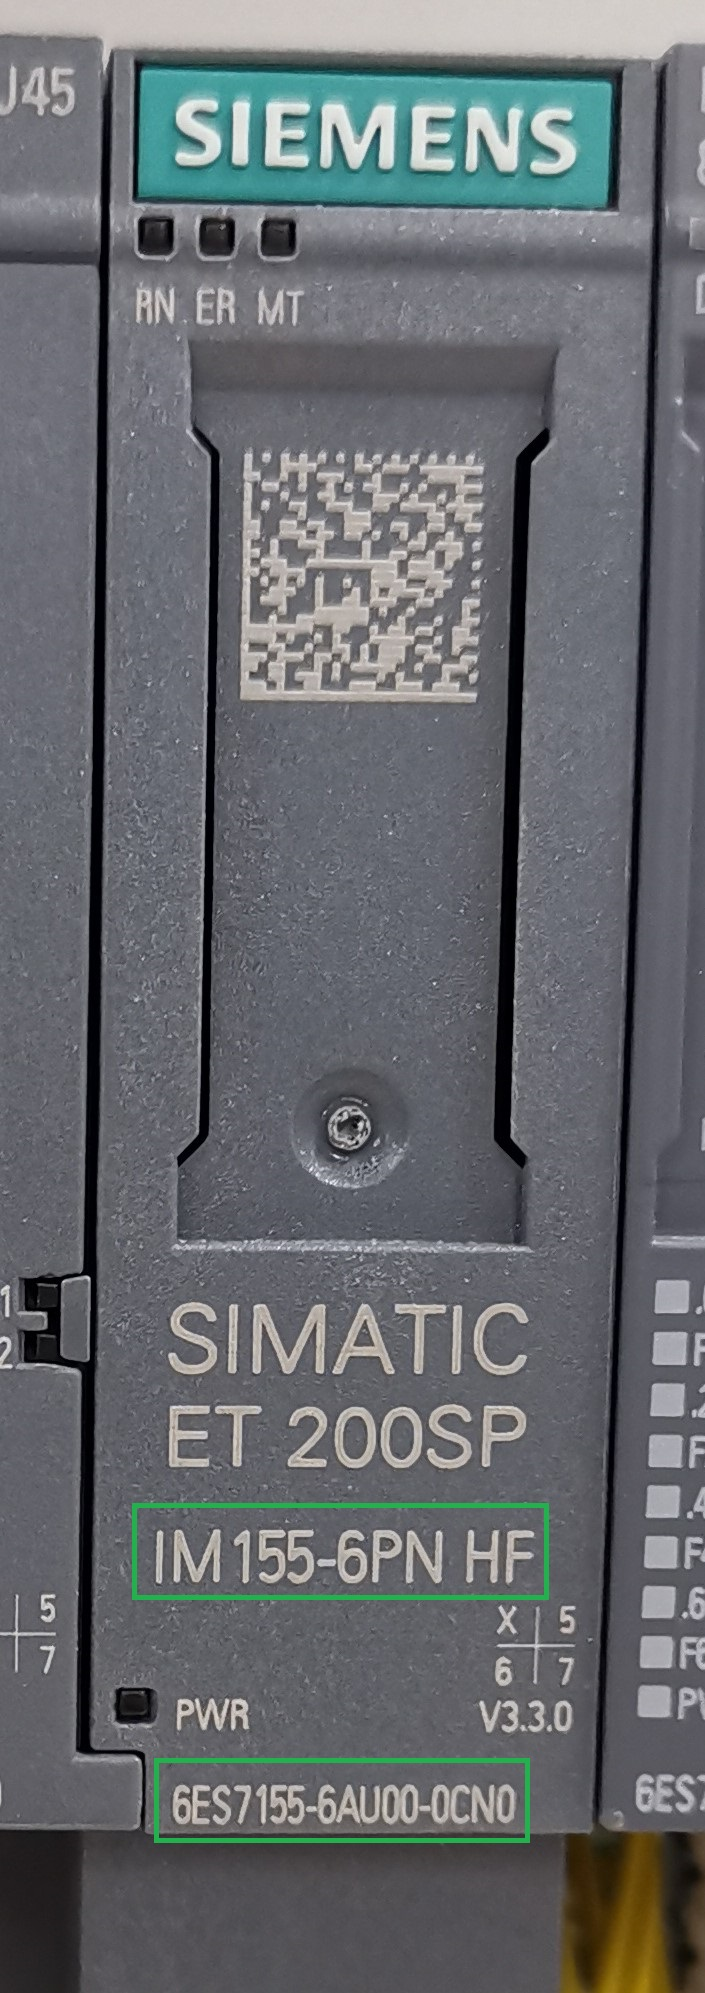
\includegraphics[width=0.4\linewidth]{Bilder/2. Inbetriebnahme/4. Konfiguration der ET 200 SP/4.1 ET 200 SP hinzufügen/(4.1.1) Modulbezeichnung am Beispiel des IM 155-Moduls.jpg}}
        \caption[Modulbezeichnung am Beispiel des IM 155-Interfacemoduls]{Modulbezeichnung am Beispiel des IM 155-Interfacemoduls}
        \label{fig:Bild6.20}
   \end{minipage}
   \hspace{.1\linewidth}% Abstand zwischen Bilder
   \begin{minipage}[b]{.4\linewidth}
        \centering
        \fbox{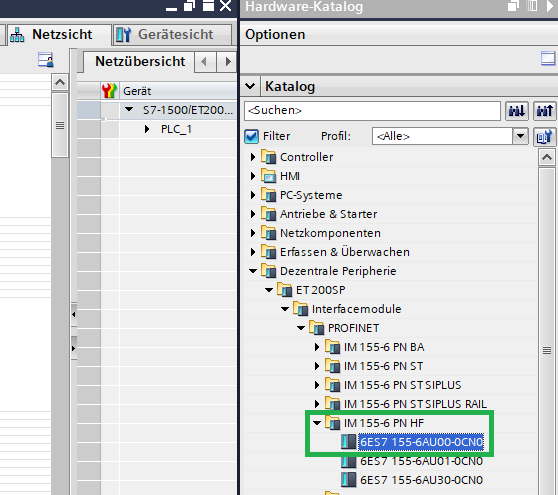
\includegraphics[width=1.0\linewidth]{Bilder/2. Inbetriebnahme/4. Konfiguration der ET 200 SP/4.1 ET 200 SP hinzufügen/(4.1.2) Dezentrale Peripherie hinzufuegen.png}}
        \caption[Dezentrale Peripherie hinzufügen]{Dezentrale Peripherie hinzufügen\\}
        \label{fig:Bild6.21}
   \end{minipage}
\end{figure}

\clearpage

\subsubsection{Module hinzufügen}
In der \textbf{Gerätesicht} der ET 200SP über den Katalog die weiteren Module hinzufügen.\\
\textbf{ACHTUNG:} Die Bezeichnungen auf den realen Modulen weichen teils von denen im TIA-Portal ab.

\begin{figure}[H]
   \centering
   \fbox{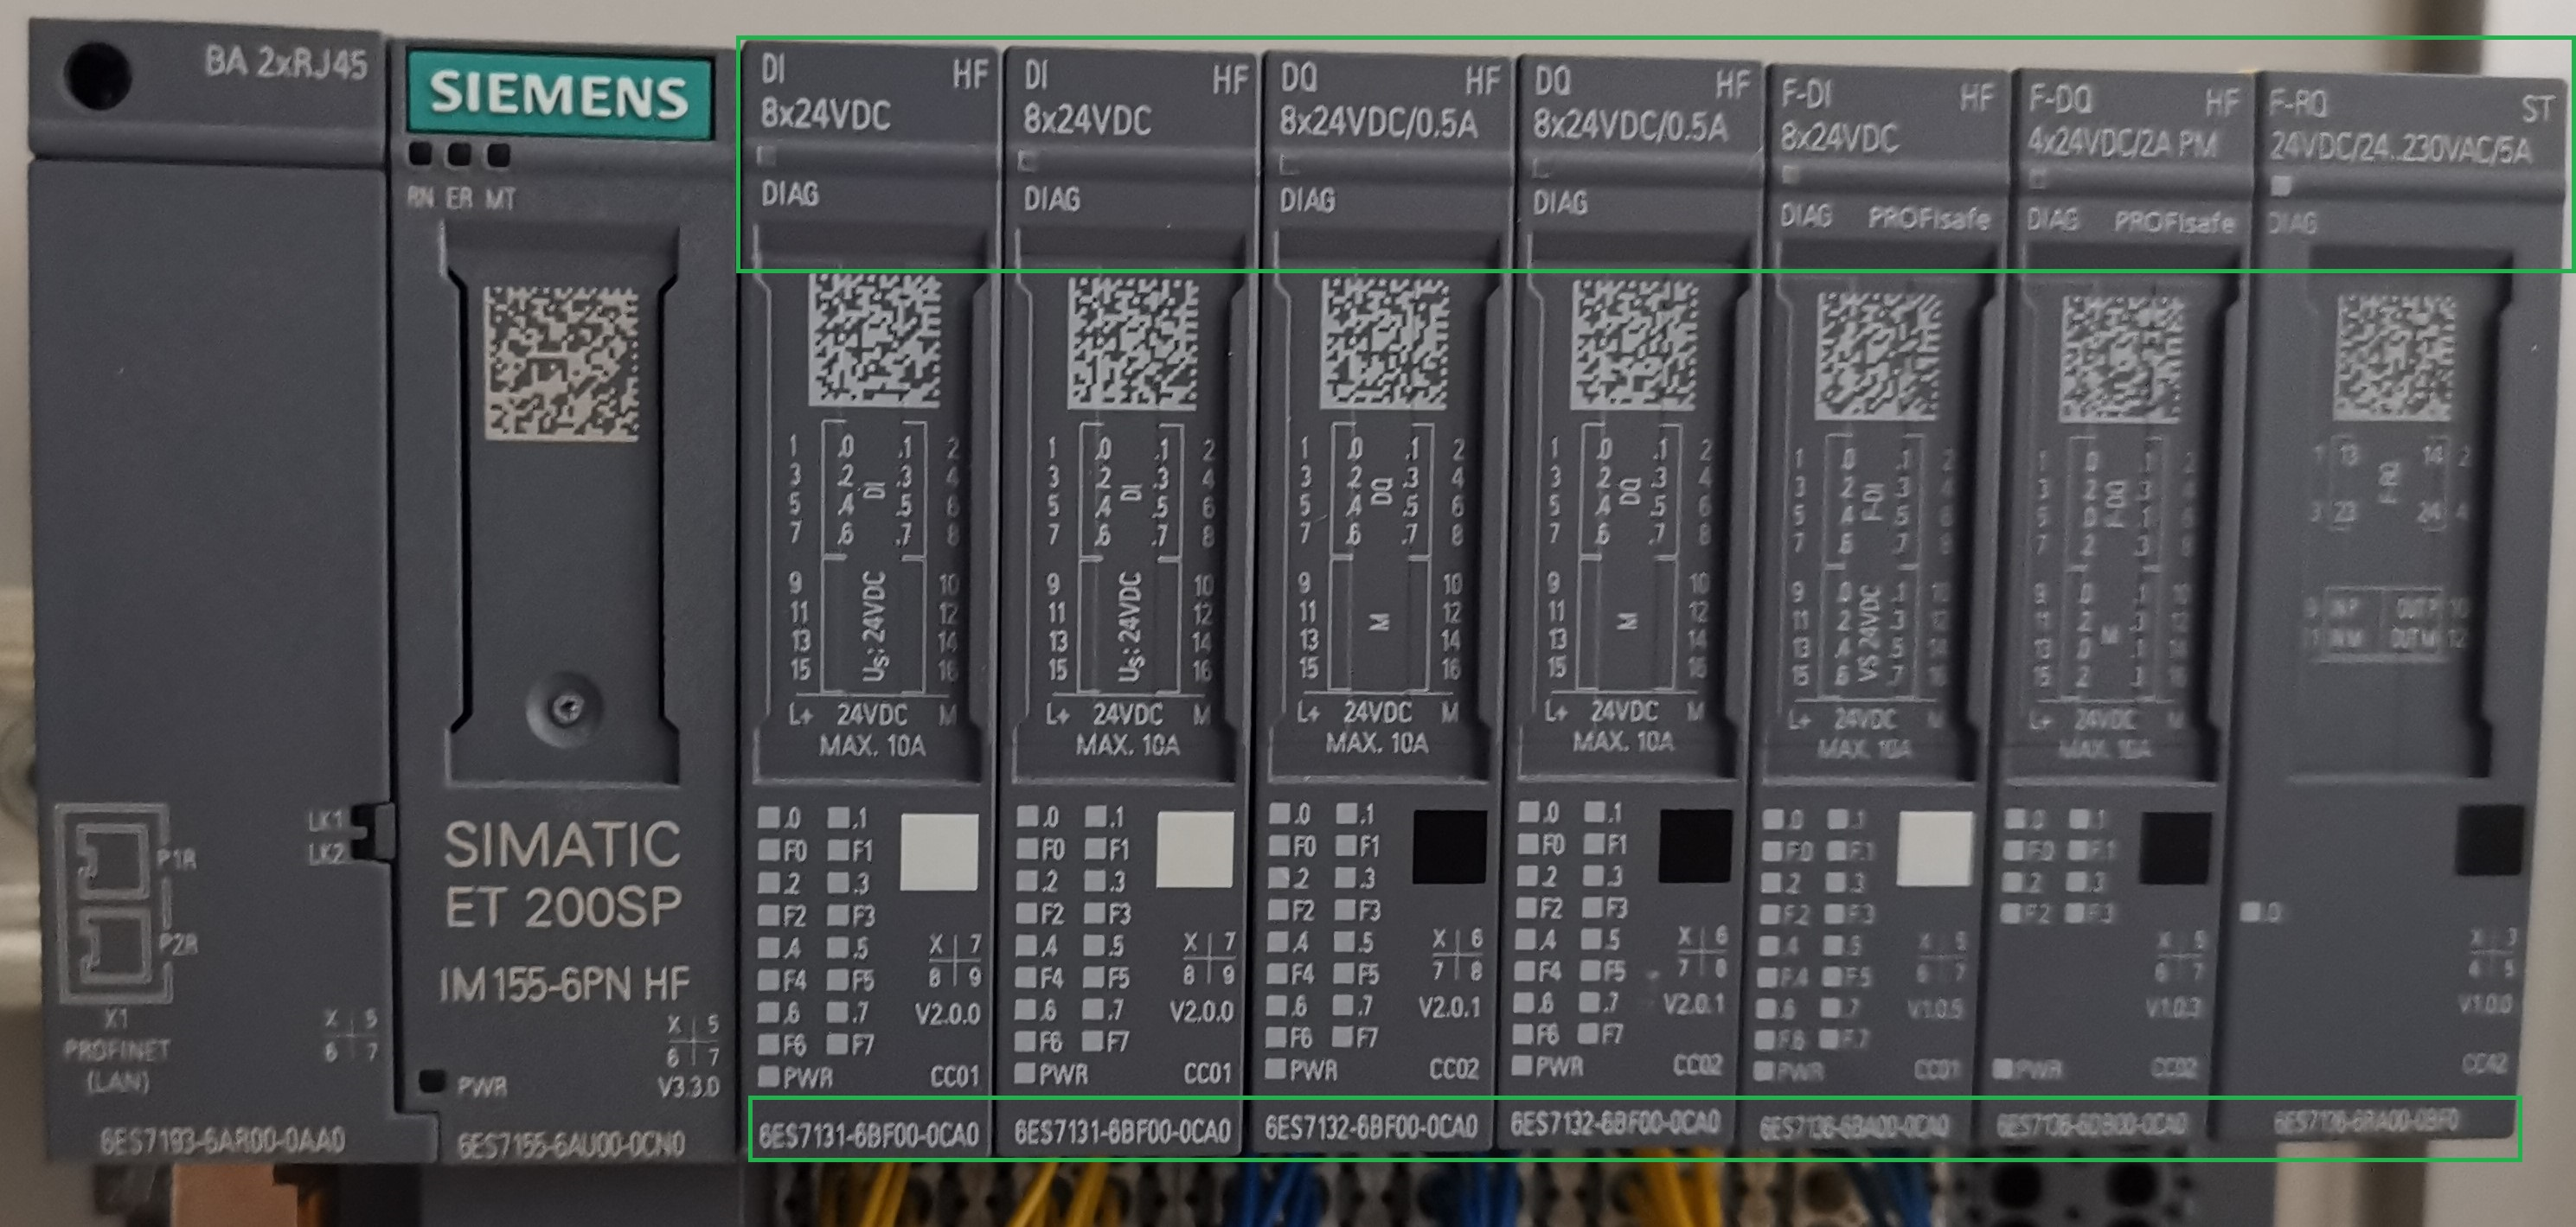
\includegraphics[width=0.9\textwidth]{Bilder/2. Inbetriebnahme/4. Konfiguration der ET 200 SP/4.2 Module hinzufügen/(4.2.1) Übersicht aller Module der dezentralen Peripherie.jpg}}
   \caption[Übersicht der Module der dezentralen Peripherie]{Übersicht der Module der dezentralen Peripherie}
   \label{fig:Bild6.22}
\end{figure}

\begin{table}[H]
    \centering
    \begin{tabular}{|c|c|c|}
        \hline
         \textbf{Modulbezeichnung} & \textbf{Modulnummer} & \textbf{Version} \\
         \hline
         DI 8x24VDC HF	& 6ES7131-6BF00-0CA0	& 2.0.0 \\
         \hline
         DI 8x24VDC HF	& 6ES7131-6BF00-0CA0	& 2.0.0 \\
         \hline
         DQ 8x24VDC/0.5A HF &	6ES7132-6BF00-0CA0	& 2.0.1 \\
         \hline
         DQ 8x24VDC/0.5A HF &	6ES7132-6BF00-0CA0	& 2.0.1 \\
         \hline
         F-DI 8x24VDC HF & 	6ES7136-6BA00-0CA0	& 1.0.5 \\
         \hline
         F-DQ 4x24VDC/2A PM HF & 	6ES7136-6DB00-0CA0	& 1.0.3 \\
         \hline
         F-RQ 24VDC/24…230VAC/5A ST & 	6ES7136-6RA00-09F0	& 1.0.0 \\
         \hline
    \end{tabular}
    \caption{Modulbezeichnungen, -nummern und -versionen}
    \label{tab:Tab6.1}
\end{table}

\begin{figure}[H]
   \centering
   \fbox{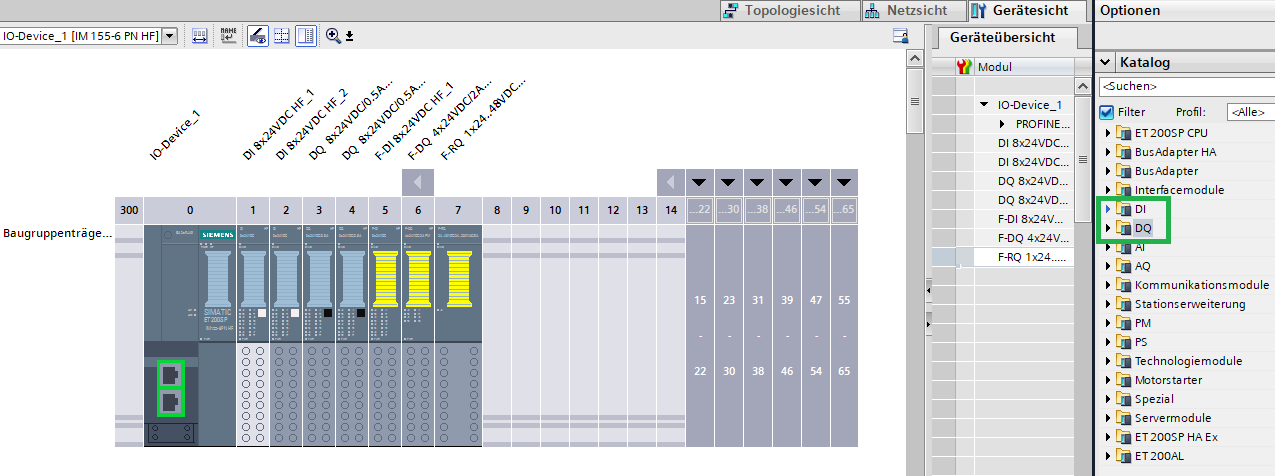
\includegraphics[width=0.9\textwidth]{Bilder/2. Inbetriebnahme/4. Konfiguration der ET 200 SP/4.2 Module hinzufügen/(4.2.2) Elemente der dezentralen Peripherie hinzufuegen.png}}
   \caption[Module hinzufügen]{Module hinzufügen}
   \label{fig:Bild6.23}
\end{figure}

Alle eingefügten Module (bis auf: F-RQ 24VDC/24…230VAC/5A ST) werden zu einer \textbf{Potentialgruppe} hinzugefügt. Dies kann durch das Anklicken der Module und dem anschließenden auswählen von \glqq\textbf{Neue Potentialgruppe ermöglichen (helle BaseUnit)}\grqq\:erfolgen.\\
Pfad: Allgemein > Potentialgruppe

\begin{figure}[H]
   \centering
   \fbox{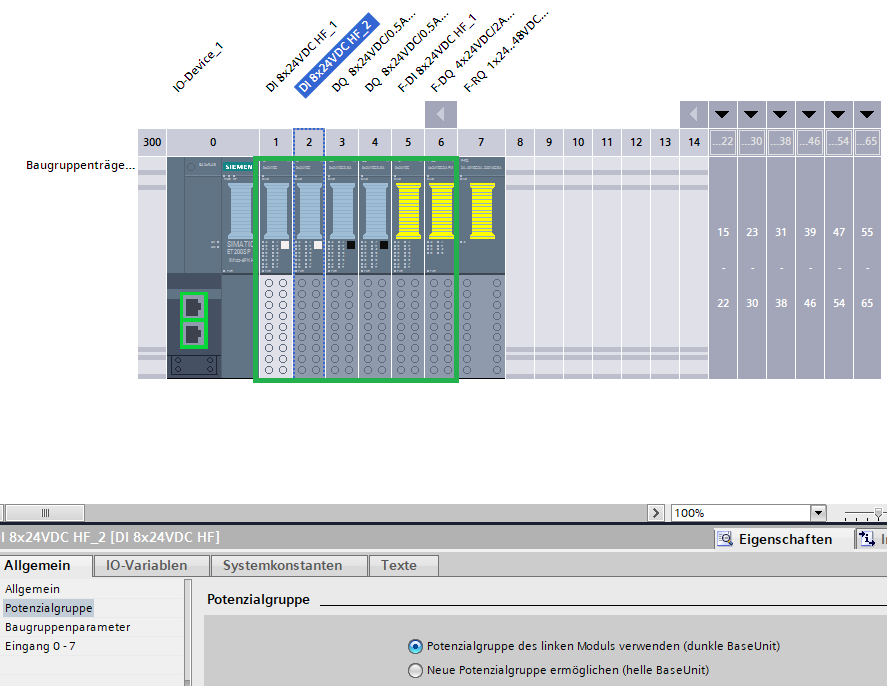
\includegraphics[width=0.75\textwidth]{Bilder/2. Inbetriebnahme/4. Konfiguration der ET 200 SP/4.2 Module hinzufügen/(4.2.3) Potenzialgruppe aendern.png}}
   \caption[Potenzialgruppe anpassen]{Potenzialgruppe anpassen}
   \label{fig:Bild6.24}
\end{figure}

\subsubsection{Geräteversionen tauschen}
Sofern dies nicht bereits beim Einfügen der Module beachtet wurde, müssen die Versionen des Interfacemoduls IM 155-6PN HF und des Moduls F-DQ angepasst werden. Dies kann durch einen Rechtsklick in der \textbf{Gerätesicht} auf das \glqq\textbf{Modul > Geräte tauschen..}\grqq\:durchgeführt werden. Die Versionsnummern siehe \autoref{tab:Tab6.1}. \\
\textbf{ACHTUNG:} Die Artikel-Nummern müssen übereinstimmen.

\begin{figure}[H]
   \centering
   \fbox{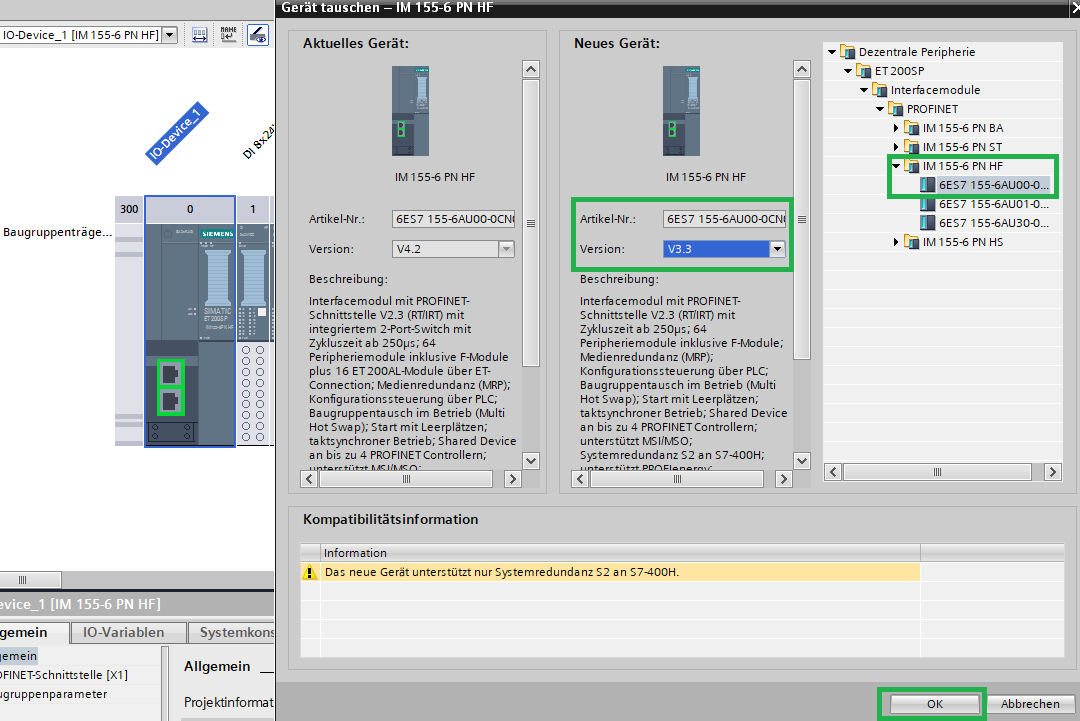
\includegraphics[width=0.65\textwidth]{Bilder/2. Inbetriebnahme/4. Konfiguration der ET 200 SP/4.3 Geräteversionen tauschen/(4.3.1) Geraeteversion tauschen.png}}
   \caption[Geräteversion des IM 155-Interfacemoduls tauschen]{Geräteversion des IM 155-Interfacemoduls tauschen}
   \label{fig:Bild6.25}
\end{figure}

\begin{figure}[H]
   \centering
   \fbox{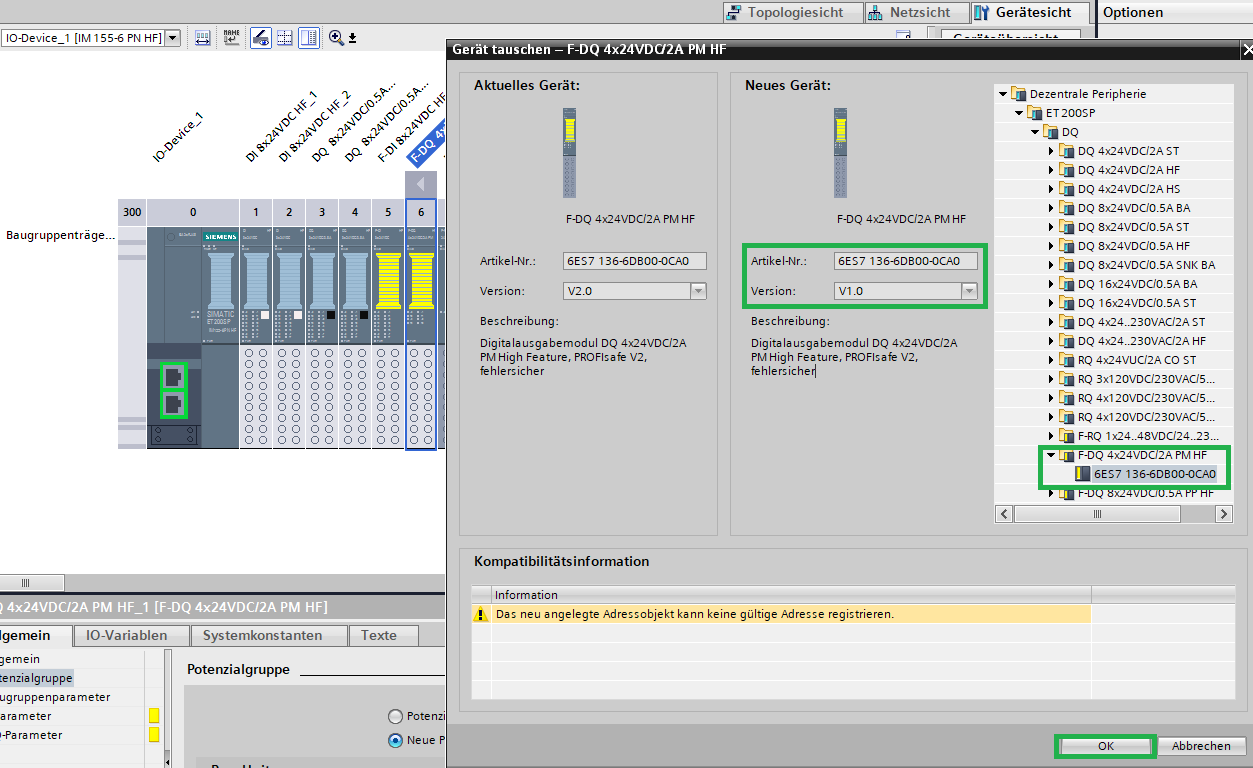
\includegraphics[width=0.65\textwidth]{Bilder/2. Inbetriebnahme/4. Konfiguration der ET 200 SP/4.3 Geräteversionen tauschen/(4.3.2) Geraeteversion tauschen.png}}
   \caption[Geräteversion des F-DQ-Moduls tauschen]{Geräteversion des F-DQ-Moduls tauschen}
   \label{fig:Bild6.26}
\end{figure}

\subsubsection{IP-Adresse und Vergabe des PROFINET-Gerätenamen der ET 200SP} \label{sec: IP-Adresse_PROFINET-Gerätename_ET_200SP}
Die Bezeichnung der PROFINET-Schnittstelle der ET 200SP ist \textbf{X1}.

\begin{figure}[H]
   \centering
   \fbox{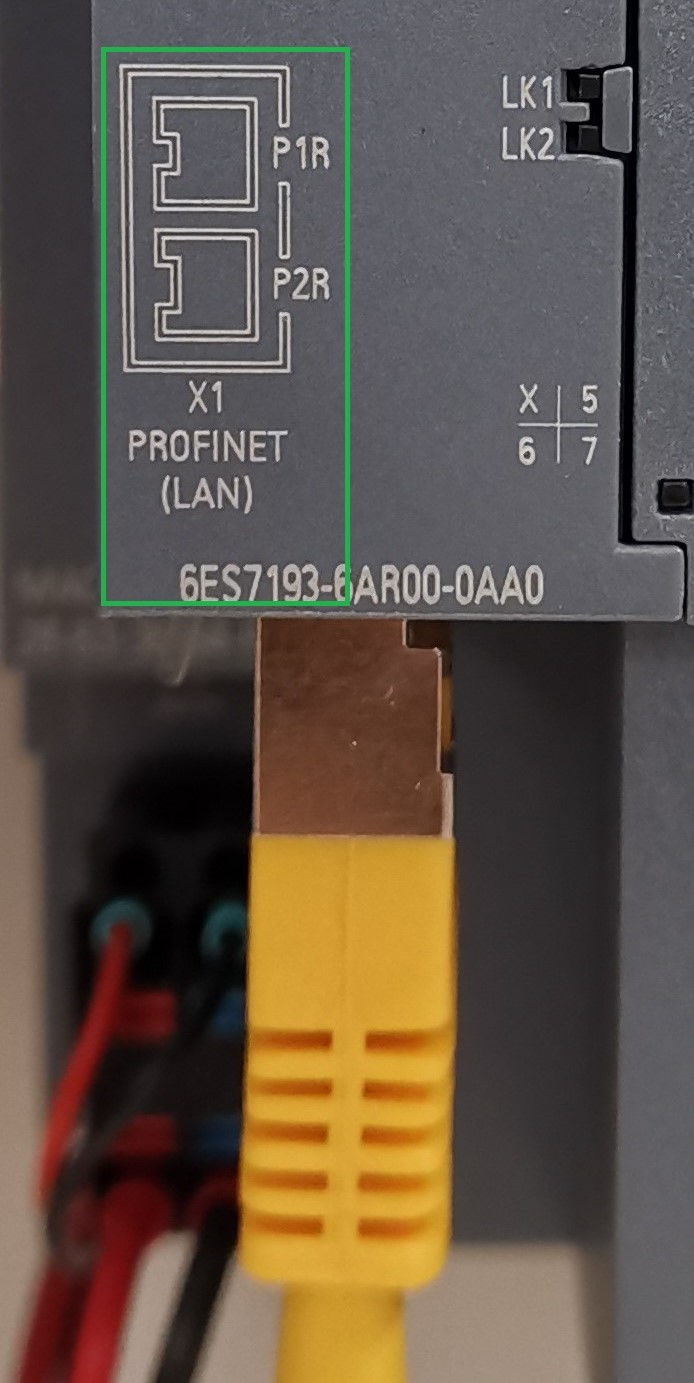
\includegraphics[width=0.2\textwidth]{Bilder/2. Inbetriebnahme/4. Konfiguration der ET 200 SP/4.4 IP-Adresse und Vergabe des PROFINET-Gerätenamen der ET 200 SP/(4.4.1) Bezeichnung der PROFINET-Schnittstelle.jpg}}
   \caption[Bezeichnung der PROFINET-Schnitstelle der ET 200SP]{Bezeichnung der PROFINET-Schnittstelle der ET 200SP}
   \label{fig:Bild6.27}
\end{figure}

Die benötigte IP-Adresse und PROFINET-Gerätename können der \autoref{fig:Bild6.3} entnommen werden. Die Einstellungen sind über die \textbf{Gerätesicht} des Gerätes ET 200SP sichtbar. Bei der Vergabe des PROFINET-Gerätenamens das Häkchen bei \glqq\textbf{PROFINET-Gerätename automatisch generieren}\grqq\:entfernen.\\
Pfad: Allgemein > PROFINET-Schnittstelle [X1]

\begin{figure}[H]
   \centering
   \fbox{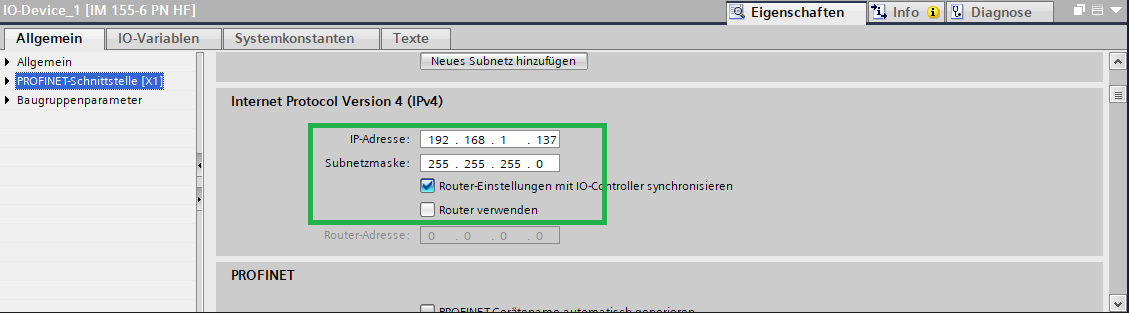
\includegraphics[width=0.95\textwidth]{Bilder/2. Inbetriebnahme/4. Konfiguration der ET 200 SP/4.4 IP-Adresse und Vergabe des PROFINET-Gerätenamen der ET 200 SP/(4.4.2) IP-Adresse der ET 200 SP.png}}
   \caption[Vergabe der IP-Adresse der ET 200SP]{Vergabe der IP-Adresse der ET 200SP}
   \label{fig:Bild6.28}
\end{figure}

\begin{figure}[H]
   \centering
   \fbox{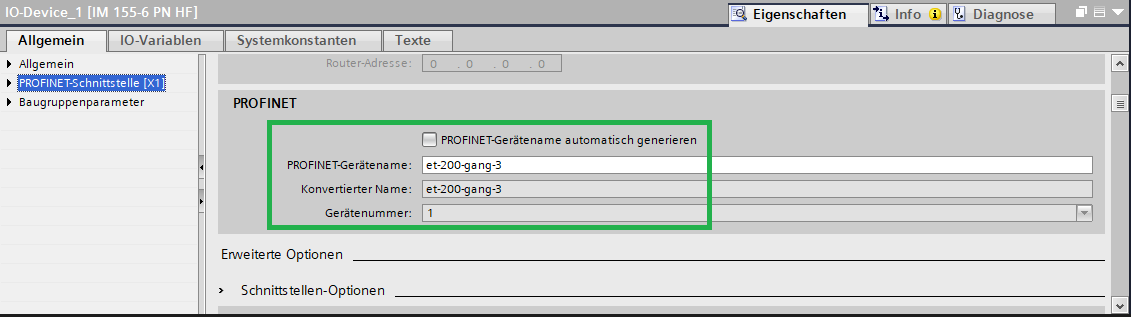
\includegraphics[width=0.95\textwidth]{Bilder/2. Inbetriebnahme/4. Konfiguration der ET 200 SP/4.4 IP-Adresse und Vergabe des PROFINET-Gerätenamen der ET 200 SP/(4.4.3) PROFINET-Geraetename der ET 200 SP.png}}
   \caption[Vergabe des PROFINET-Gerätenamen der ET 200SP]{Vergabe des PROFINET-Gerätenamen der ET 200SP}
   \label{fig:Bild6.29}
\end{figure}

\clearpage

\subsection{PROFINET-Verbindung} \label{sec:ergebnisse}

\subsubsection{Verbindung herstellen} \label{sec: Verbindung herstellen}
Die PROFINET-Verbindung beider Geräte und deren Module wird über die \textbf{Netzsicht} vorgenommen. Dabei ist auf die richtigen Anschlüssen zu achten (s. \autoref{sec: IP-Adresse_PROFINET-Gerätename_S7-1500} und \autoref{sec: IP-Adresse_PROFINET-Gerätename_ET_200SP}).

\begin{figure}[H]
   \centering
   \fbox{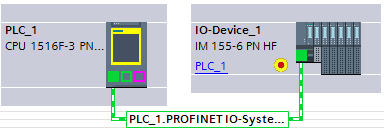
\includegraphics[width=0.8\textwidth]{Bilder/2. Inbetriebnahme/5. PROFINET-Verbindung/5.1 Verbindung herstellen/(5.1.1) PROFINET-Verbindung ziehen.png}}
   \caption[PROFINET-Verbindung herstellen]{PROFINET-Verbindung herstellen}
   \label{fig:Bild6.30}
\end{figure}

\subsubsection{Fehlersicherheit aktivieren}
Zusätzlich zur PROFINET-Verbindung in der Netzsicht ist in den Einstellungen der S7-1500 (über \textbf{Gerätesicht}) die Fehlersicherheit (\textbf{F-Fähigkeit}) zu aktivieren.\\
Pfad: Fehlersicherheit > F-Aktivierung

\begin{figure}[H]
   \centering
   \fbox{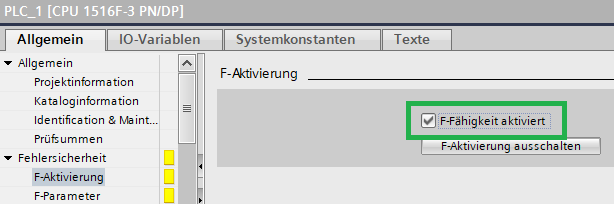
\includegraphics[width=0.8\textwidth]{Bilder/2. Inbetriebnahme/5. PROFINET-Verbindung/5.2 Fehlersicherheit aktivieren/(5.2.1) Fehlersicherheit aktivieren.png}}
   \caption[Fehlersicherheit aktivieren]{Fehlersicherheit aktivieren}
   \label{fig:Bild6.31}
\end{figure}

\subsubsection{Überprüfung des internen PROFINET-Gerätenamens der ET 200SP}
Möglicherweise stimmt der intern festgelegte Gerätename nicht mit dem nach \autoref{sec: IP-Adresse_PROFINET-Gerätename_ET_200SP} vergebenen überein. Um dies zu kontrollieren, kann über einen Rechtsklick auf die gesetzte PROFINET-Verbindung in der Netzsicht (s. \autoref{sec: Verbindung herstellen}) der Gerätename der ET 200SP ausgelesen und abgeglichen werden (\textbf{Rechtsklick > Gerätename zuweisen})(\autoref{fig:Bild6.32}).  Stimmen die Gerätenamen nicht überein, muss der Name entsprechend geändert werden (s. \autoref{sec: IP-Adresse_PROFINET-Gerätename_ET_200SP}).

\begin{figure}[H]
   \centering
   \fbox{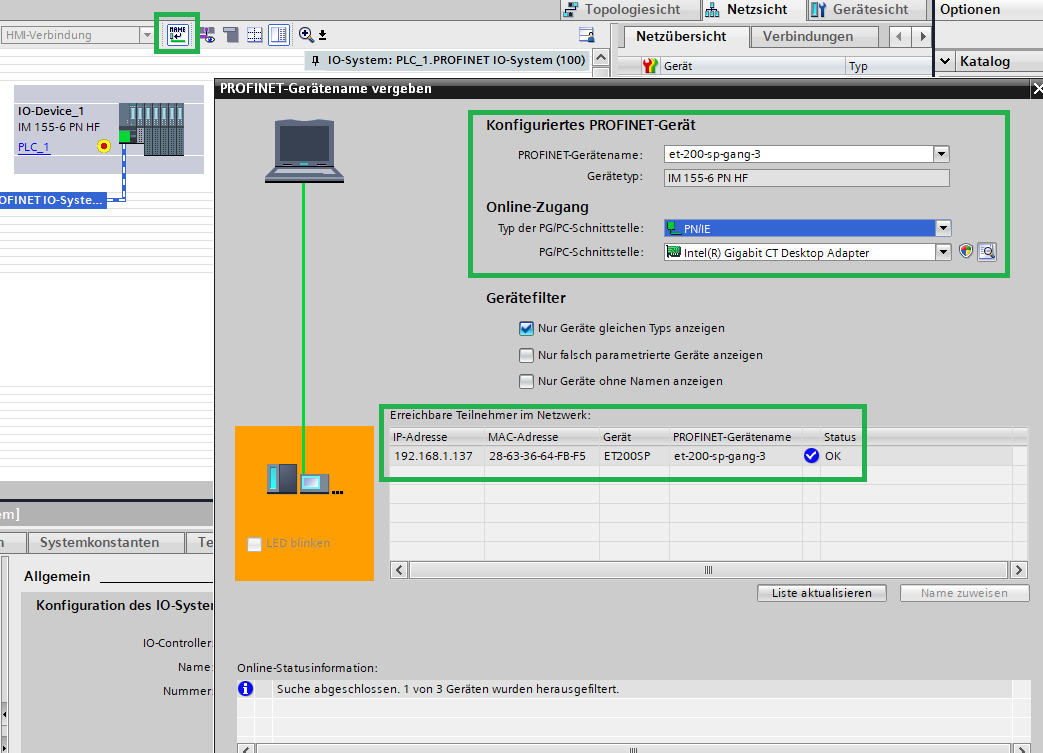
\includegraphics[width=0.8\textwidth]{Bilder/2. Inbetriebnahme/5. PROFINET-Verbindung/5.3 Überprüfung des internen PROFINET-Gerätenamens der ET 200SP/(5.3.1) Ueberpruefung der richtigen Namen.png}}
   \caption[Überprüfung des internen Gerätenamens der ET 200SP]{Überprüfung des internen Gerätenamens der ET 200SP}
   \label{fig:Bild6.32}
\end{figure}

\subsubsection{Überprüfung der IP-Adressen der Geräte}
Eine weitere Überprüfung für die korrekte Verbindung ist in der Netzsicht über den Button \glqq\textbf{Adressen anzeigen}\grqq\:möglich. Hierbei werden die IP-Adressen der Geräte angezeigt. Diese können mit der \autoref{fig:Bild6.3} abgeglichen werden. Sofern keine Verbindung hergestellt wurde, wird eine Fehlermeldung ausgegeben.

\begin{figure}[H]
   \centering
   \fbox{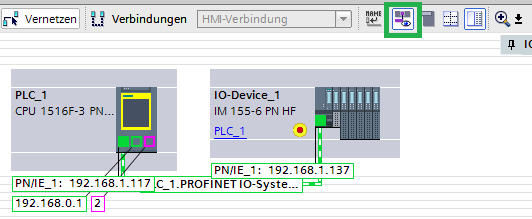
\includegraphics[width=0.8\textwidth]{Bilder/2. Inbetriebnahme/5. PROFINET-Verbindung/5.4 Überprüfung der IP-Adressen der Geräte/(5.4.1) Ueberpruefung der richtigen Adressen.png}}
   \caption[Überprüfung der IP-Adressen der Geräte]{Überprüfung der IP-Adressen der Geräte}
   \label{fig:Bild6.33}
\end{figure}

\clearpage

\subsection{Laden und Übersetzen der Hard- und Software} \label{sec: laden_und_uebersetzen}

Bevor eine Online-Verbindung mit der SPS aufgebaut werden kann, wird die Hard- und Software übersetzt (\autoref{fig:Bild6.34}) und anschließend in das Gerät geladen (\autoref{fig:Bild6.35}).

\begin{figure}[H]
   \centering
   \fbox{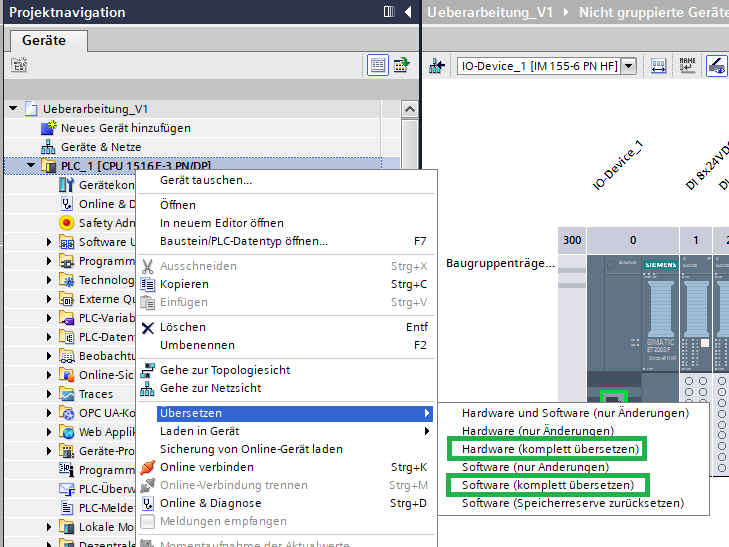
\includegraphics[width=0.6\textwidth]{Bilder/2. Inbetriebnahme/6. Laden und Übersetzen der Hard- und Software/(6.1) Uebersetzen.PNG}}
   \caption[Übersetzen der Hard- und Software]{Übersetzen der Hard- und Software}
   \label{fig:Bild6.34}
\end{figure}

\begin{figure}[H]
   \centering
   \fbox{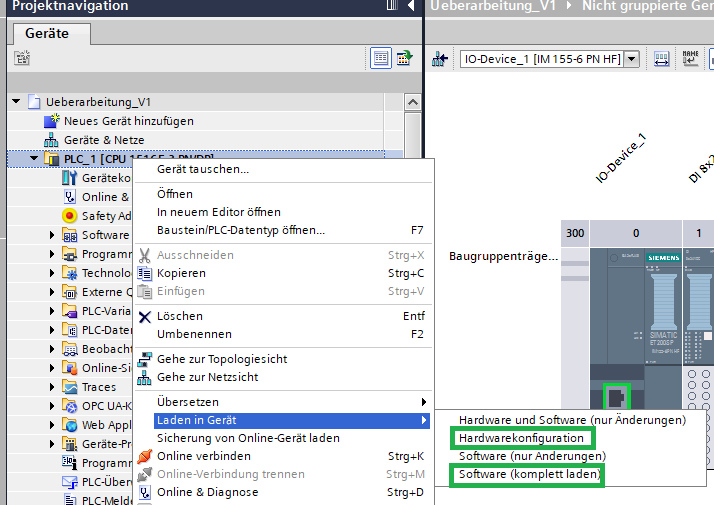
\includegraphics[width=0.6\textwidth]{Bilder/2. Inbetriebnahme/6. Laden und Übersetzen der Hard- und Software/(6.2) Laden.PNG}}
   \caption[Laden der Hard- und Software]{Laden der Hard- und Software}
   \label{fig:Bild6.35}
\end{figure}

\clearpage

\subsection{Vergabe der PROFIsafe-Adressen} \label{sec: vergabe der profisafe-adressen}

Nachdem die Online-Verbindung über \glqq\textbf{Online verbinden}\grqq\:hergestellt wurde, müssen die PROFIsafe-Adressen der F-DI und der F-DQ-Module vergeben werden. Dies kann durch einen \textbf{Rechtsklick auf Modul > PROFIsafe-Adresse zuweisen} durchgeführt werden. Anschließend wird das Menü aus \autoref{fig:Bild6.36} geöffnet. Nach Eingabe der Einstellungen des Online-Zugangs wird über \glqq\textbf{Identifikation}\grqq\:das entsprechende Modul ausgewählt. Durch das Setzen des Häkchen bei \glqq\textbf{Bestätigen}\grqq\:und dem Drücken von \glqq\textbf{PROFIsafe-Adresse zuweisen}\grqq\:wird die Einstellung übernommen.

\begin{figure}[H]
   \centering
   \fbox{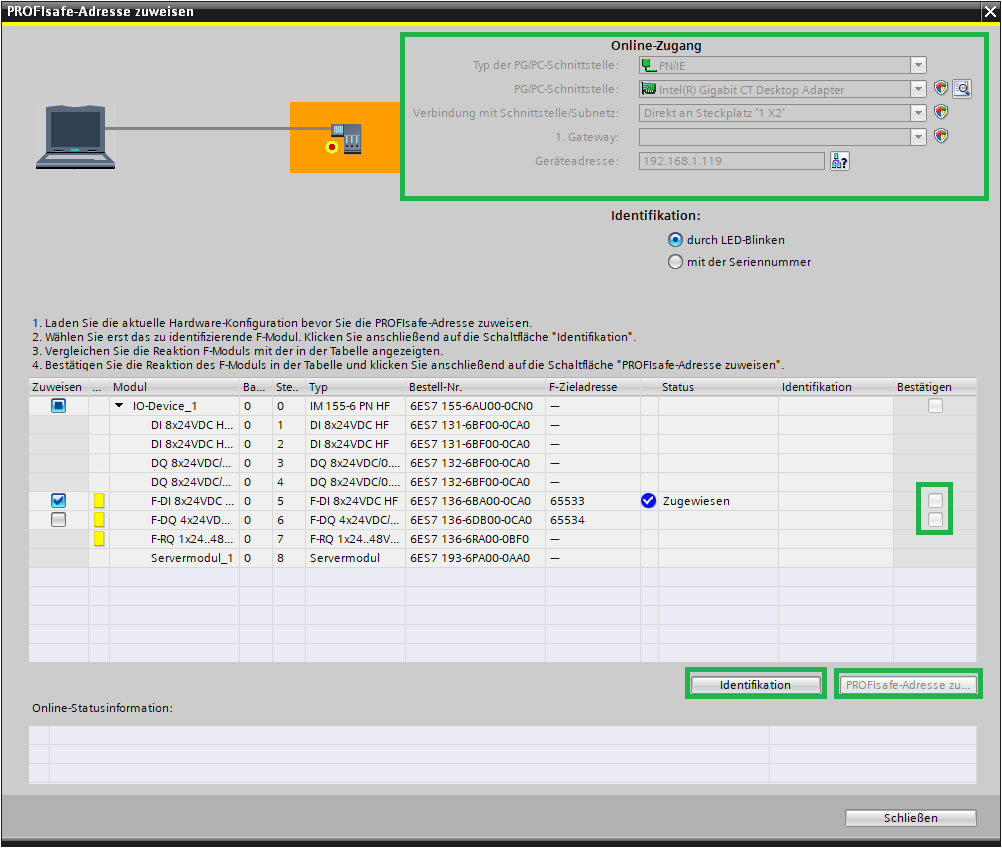
\includegraphics[width=0.95\textwidth]{Bilder/2. Inbetriebnahme/7. Vergabe der PROFIsafe-Adressen/(7.1) Vergabe der PROFIsafe-Adressen.PNG}}
   \caption[Vergabe der PROFIsafe-Adressen]{Vergabe der PROFIsafe-Adressen}
   \label{fig:Bild6.36}
\end{figure}


%---------Quellen---------------------------------
\newpage
\newcount\Quellennummer
\Quellennummer=1

\renewcommand\refname{Literaturverzeichnis}
\addcontentsline{toc}{section}{Literaturverzeichnis}

\begin{thebibliography}{999}
{\setlength{\emergencystretch}{3cm}%

\bibitem[\the\Quellennummer]{HTWgross}
HTW-Logo auf dem Deckblatt\par
\url{https://de.wikipedia.org/wiki/Datei:Logo_HTW_Berlin.svg} \par
 Stand: 17.08.2018 um 14:49 Uhr

\advance\Quellennummer by 1
 
\bibitem[\the\Quellennummer]{HTWklein}
HTW-Logo in der Kopfzeile\par
\url{http://tonkollektiv-htw.de/} \par
 Stand: 17.08.2018 um 14:53 Uhr

\advance\Quellennummer by 1

}
\end{thebibliography}

\end{document}
